% !BIB TS-program = 
%%%%%%%%%%%%%%%%%%%%%%%%%%%%%%%%%

% This is the "before the document" area, where to define parameters for the cover sheet and to include libraries

%%%%%%%%%%%%%%%%%%%%%%%%%%%%%%%%%

\documentclass[11pt]{article} 

%libraries
\usepackage{geometry}
\usepackage{float}
\usepackage{amsmath}
\usepackage{mathtools}
\usepackage{url}
\usepackage{amssymb}
\usepackage{amsmath}
\usepackage{units}
\usepackage{siunitx}
\usepackage{fancyhdr}
\usepackage{graphicx}
\usepackage{multicol}
\usepackage{setspace}
\usepackage{listings}
\usepackage[numbered,autolinebreaks,useliterate]{mcode}
\usepackage{pdfpages}
\usepackage{booktabs} 
\usepackage{bigstrut}
\usepackage{bigdelim}
\usepackage{subcaption}
\usepackage{multirow}
\usepackage[nottoc]{tocbibind}
\usepackage{rotating}
\usepackage[parfill]{parskip}
\usepackage[utf8]{inputenc}
\usepackage[english]{babel}
\usepackage{comment} 

%pagestyle
\geometry{paper=a4paper,left=30mm,right=25mm,top=40mm,bottom =30mm,headsep=20mm}

\pagestyle{fancy}
\fancyhf{}


%%%%%%%%%%%%%%%%%%%%%%%%%%%%%%%%%

% Header and Footer

%%%%%%%%%%%%%%%%%%%%%%%%%%%%%%%%%

%Kopfzeile links bzw. innen
\fancyhead[L]{\large{}}
%Kopfzeile mittig
\fancyhead[C]{\large{Master Thesis}}
%Kopfzeile rechts bzw. außen
%\fancyhead[R]{
\includegraphics{files/TUs}}
%Linie oben
\renewcommand{\headrulewidth}{0.5 pt}

%Fußzeile mittig
\fancyfoot[C]{\thepage}


%%%%%%%%%%%%%%%%%%%%%%%%%%%%%%%%%

% Titlepage

%%%%%%%%%%%%%%%%%%%%%%%%%%%%%%%%%

%Now we start the main document body
\begin{document}
\sloppy

\begin{titlepage}
	\begin{multicols}{2} 
		\textbf {Technische Universit\"{a}t Berlin}\\
		Faculty:            \\ Geodesy and Geoinformation Science\\  \\
		Professor: \\
		Dr. Martin Kada\\
		\columnbreak
		\flushright
		
\includegraphics{files/TU} 
	\end{multicols}

	%Absatz
	\vspace{0.1\textheight}
	
	%Absatz
	\begin{verbatim}
 
 
 
	\end{verbatim}
	\begin{center}
		\textbf{\Large{Master Thesis: \\[1 cm] Lunar Crater Detection via Deep Learning and its Application for Age Estimation}}
	\end{center}
	\vspace{0.25\textheight}
	\begin{center}
		\vspace{0.7cm}
		\textbf{Author:}\\
		Tahir, Waqas \\
	\end{center}
	\begin{center}	
		\textbf{Supervisors:}\\
		Agoub, Amgad\\
		Gläser, Philipp
	\end{center}
	\begin{verbatim}
	\end{verbatim}
	\begin{center}
		\today
	\end{center}

\end{titlepage}

%this command is used in order to have every section in a different page, but avoid to use it!
\newpage 


%%%%%%%%%%%%%%%%%%%%%%%%%%%%%%%%%

% Table of Contents

%%%%%%%%%%%%%%%%%%%%%%%%%%%%%%%%%

%create the table of contents, figures and tables
\tableofcontents

\newpage
%%%%%%%%%%%%%%%%%%%%%%%%%%%%%%%%%

% Sections and Subsections

%%%%%%%%%%%%%%%%%%%%%%%%%%%%%%%%%

\iffalse

\section{Deep learning}


\par

\section{Supervised learning}

\par
The weight vector needs to be adjusted. The learning algorithm computes a gradient in the form of a vector for each weight which indicates the increment or decrement in error by increasing tiny amount of weight. The adjustment of weight vector is made in the opposite direction of the gradient vector. \cite{lecun_deep_2015-2}

\par
A procedure known as stochastic gradient descent is widely used by practitioners. In this procedure an input vector is shown for some examples then outputs, average gradient and errors are computed and weights are adjusted accordingly. This process is iterated for small set of multiple examples taken from training data set until the average of objective function does not further decrease. After training, the machine's performance ability is measured by feeding a test data set. This is completely new data set to machine and it produces sensible outputs from the input that it has not seen during training.

\section{Modern History of Object Detection}
Object detection has greatly inproved over the last few years. The era of deep learning had a major breakthrough when ~\cite{zhevsky_imagenet_2012} won the ImageNet  \cite{lecun_deep_2015} 

\section{Cut lines}
Keeping in view the achievements of Mask R-CNN over previously developed algorithms, we decided to test this algorithm on lunar crater dataset. The dataset consists of 4 million images. Figure \ref{fig:Mask R-CNN results on the COCO test set.} shows the result of Mask R-CNN on COCO dataset. Faster R-CNN was extended for pixel level segmentation.

\par
Machine learning methodology becomes handy over classical object detection approaches when it comes to detecting objects from different datasets on which algorithm was not trained. In classical computer vision methods, the images are needed to be ---------- Machine learning algorithm requires labeling on of the dataset. 


\section{Introduction}
Studying impact craters present a valuable information about the geology of planets and characteristics of the surface.

\par
 Small and shallow craters can be analyzed from the images with high incidence angle (\textgreater70°).

\par
One single image taken from LRO could have several craters of different diameters. Manual detection takes a lot of time and man power with required skills. In last two decades, detecting craters manually was no longer an optimal solution because of several reasons like as mentioned earlier, manual detection of craters is a laborious work with involvement of man power. Another major drawback is that only qualified individuals can perform detection process. When technology is advanced enough that this laborious task can be handed over to a machine then implementing an algorithm for the automatic detection of craters would not only save time but also dependency on skilled individuals to carry out this task. 

\par
Earlier this decade, development in computer graphical units made it possible to process big data. This created an opportunity for scientists to test machine learning architectures for object detection. Convolutional neural networks also known as CNNs or ConvNets are an architecture of supervised machine learning model that have proved their success by winning Large Scale Visual Recognition Challenge (ILSVRC-2010) competition which was composed of 1.2 million high-resolution images. \cite{krizhevsky_imagenet_2012} achieved top-1 and top-5 error rates of 37.5\% and 17.0\% respectively. This success gave rise to ConvNets architectures and since then scientists have been working to increase the object classification speed of such algorithms.

The aim is to develop a CNN architect and test its performance on automatically crater presence and edge detection by performing a series of computations. Mask R-CNN (Mask Region Convolutional neural network) was presented in 2017 where the goal was a pixel level classification of each pixel into fixed set of categories. The example image of such method is shown in figure \ref{fig:Mask R-CNN results on the COCO test set.}. Other than CNNs, there is another way to detect an object, YOLO (You Look Only Once) i.e. does not classify objects as accurately as CNN because in YOLO each object in the image is assigned to grid cell that contains the object's midpoint. Each grid detects one object only regardless the number of bounding boxes. It is faster than CNN because it takes object detection as a regression problem to spatially separated bounding boxes and class probabilities associated with it, these classes are predicted with a single neural network in one evaluation. One of the example of YOLO result is also shown in Figure  \ref{fig:YOLO running on sample artwork and natural images from the internet.}.

\begin{figure}[H]
	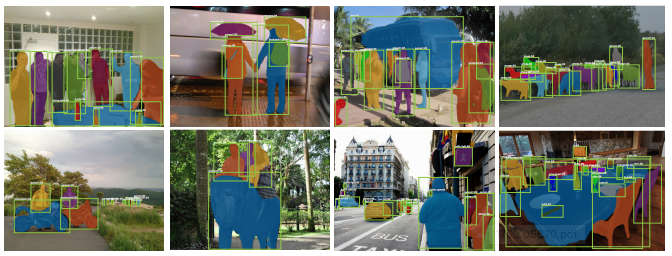
\includegraphics[width=\linewidth]{files/mask_R-CNN/results.jpg}
	\caption{Mask R-CNN results on the COCO test set.}
	\label{fig:Mask R-CNN results on the COCO test set.}
\end{figure} 

\begin{figure}[H]
	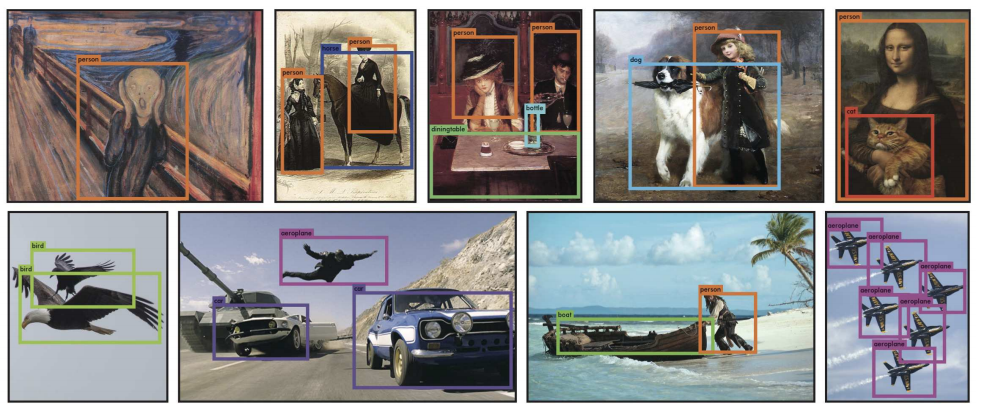
\includegraphics[width=\linewidth]{files/yolo/results.jpg}
	\caption{YOLO running on sample artwork and natural images from the Internet.}
	\label{fig:YOLO running on sample artwork and natural images from the internet.}
\end{figure}

Figure \ref{fig:YOLO running on sample artwork and natural images from the internet.} shows YOLO results on Picasso and People-Art datasets. In this image it can be seen that YOLO has predicted a person as an airplane. Even though it is mostly accurate.
\fi

\section{Introduction}
Analysis of surface of other planets is a source of learning about our own planet. Studying impact craters present a valuable information about the geology of planets and characteristics of the surface. How crater impacts can affect the life on Earth, climatic change globally and possible consequences of extreme environmental disaster. It is a known fact that solid planet surfaces are covered with tremendous amount of craters of various sizes and shapes \cite{melosh1988rocky}. Largely they form as a result of meteoroid impacts and also considered as windows into the interiors of solid planets \cite{honda2000crater}. Computation of crater density has provided a gateway for the establishment of evolution of planet surfaces chronologically \cite{martins2009crater}. This study provides not only the information about geological processes of the planet but also the history of our solar system. Knowledge of the lunar surface features including craters is vital for safe landing on Moon \cite{ivanov2015probabilistic}. According to geologists, impact craters are one of the major modifying and surface forming processes for other planets and moons of all the planets \cite{koeberl1994african}. Impact craters have also been a useful source of information for planetary scientists in providing the relative age of surfaces. Finding age from crater-counts is a commonly accepted method. Therefore, crater-counts provide a much less expensive way to find out the age of surface as compared to radioactive Age-Dating. As for the second, a rock sample is needed and age can only be determined for a specific area. Whereas by crater-counts, it is possible to find out the age of a larger area. If the relationship between the crater size and the impact energy is known then craters with larger densities indicate older surfaces \cite{ivanov2002comparison}. Despite the importance of crater and tremendous amount of data available, for decades crater analysis remained dependent on human vision and manual operation \cite{honda2000crater}.

Various processes alter crater populations especially craters with smaller diameters of only few meters. This phenomena occurs more often in planets which have dense atmosphere. These processes frequently alter crater size-frequency distributions(CSFD) \cite{opik1965mariner}. Such processes are: deceleration, ablation, fragmentation of meteors while passing through the atmosphere prior to surface impact and postformation modification of craters by erosion and deposition. Therefore, crater counts with relatively smaller diameter (i.e. diameter $<$ \SI{0.01}{\kilo\metre}) are at a larger risk of representing an age which could be misinterpreted if the modeled production function does not take into account the factors responsible for altering CSFD in an observed range of diameter \cite{hartmann1981chronology}. Moreover, several factors may lead to surface age as well as statistical uncertainties because identification of small craters is prone to certain biases such as resolution limits, illumination effects, compact crater count areas or limited number of craters \cite{soderblom1970distribution}.

In case of Earth's Moon, modeling of impact craters depends on the knowledge of age-dated lunar samples with correlation to observed CSFDs \cite{williams2018dating}. Chronology is a system composed of two elements such as a production function describing the shape of CSFD and a chronology function which is related to the accumulation of crater densities to absolute time. Both of these functions collectively provide a predicted CSFD or isochron for a given time length a surface has been under crater strikes. This is valid for the lunar surface since the Moon has no atmosphere. This chronology can also be applied to other solar system objects but with an addition of factor such as surface gravity \cite{ivanov2002comparison}. Two of such production functions are given by Hartmann and Neukum which provide an approximate surface age of the Moon. These functions are discussed in 'Related Work' section. Crater counts provide the frequency of crater distribution of a certain area. This is usually performed by counting craters manually. This task is not only time consuming but also expensive and labor intensive depending upon the number of images and amount of craters present in images. Moreover, this approach is not practical when dealing with a large amount of images with craters of various sizes on either Moon or any other planet. 

%By measuring the CSFD and diameter of craters, the age of the lunar surface can be determined using both of these parameters. It is only possible to determine the age of the same area where crater count has been performed. There are production functions proposed by planetary scientists which provide an approximation to surface age if CSFD and crater diameters are known. The examples of such functions are Hartmann Production Function (HPF) and Neukum Production Function (NPF).

Satellites carrying cameras are the source for images which provide opportunity to count craters. Since early 2000 many missions and satellites have been deployed to the Moon for research purposes including crater studies. Lunar Reconnaissance Orbiter (LRO) is a robotic mission operated by the USA that is set out to map lunar surface. It was launched in 2009 and since then it has collected a treasure trove of data. The Lunar Reconnaissance Orbiter Camera (LROC) was specifically designed for the assessment of meter-scale and smaller features to help carry out safety analysis for future lunar landing sites on the Moon including polar region. The Narrow Angle Cameras (NACs) mounted on LRO are able to detect craters with diameters of \SI{2.5}{\metre} or greater \cite{robinson2010lunar}. It is common to find craters less than \SI{100}{\metre} in diameter on the lunar surface \cite{robinson2010lunar}. These images can be utilized to count craters.

The LRO image data is available publicly and can be downloaded or viewed online \footnote{http://wms.lroc.asu.edu/lroc/}. A single image taken by the LRO requires more than \SI{150}{MB} of hard disk space. Such images cannot be processed without a competitive machine. There are methods developed to perform image processing tasks which are highly dependent on a machine's memory and performance. Therefore, developing techniques without advancement in computer technology was simply not enough. This problem was already known during the 1960s and therefore it leads to the development of Graphical processing unit (GPU). A GPU performs quick math calculations and frees the space for CPU to do other tasks. Unlike CPU, it has thousands of cores designed for multi-tasking. A much needed hardware to perform computationally expensive calculations without exhaustion. 

In the 2000s many companies like Intel, Nvidia and AMD/ATI stepped into the race of manufacturing faster GPUs and dominated the market. This competition continues till today and GPUs are becoming more and more powerful. Meanwhile, the need for GPUs is also increasing because of big data processing needs. Nvidia introduced a chip (the Ge-Force 3) capable of programmable pixel shaders i.e. compute color, position, depth or stencil of a pixel. A short program could now process each pixel before projecting it to the screen, this processing included but was not limited to the addition of image textures. By 2002 ATI Radeon 9700 the world's first Direct3D 9.0 accelerator was introduced by Microsoft containing support for multiple render targets, floating point texture formats, multiple-element textures and stencil buffer methods. In 2010 Nvidia began a partnership with Audi to power car dashboards. This mainly increased the functionality of navigation and entertainment systems. In 2014 the PS4 and Xbox One were released powered by GPUs based on AMD's Radeon HD 7850 and 7790. Lately RTX was released by Nvidia with the aim of enabling real time ray tracing. This was a new development in computer graphics for generation of interactive images reacting to lighting, reflections and shadows. RTX also includes Artificial Intelligence (AI) integration like enhancing video processing, graphics and images directly into applications. Today, parallel GPUs are making complex computations in the fields of oil exploration, machine learning, image processing, 3D reconstruction, statistics and even in the stock market for stock rate determinations.

With this advancement in computer processing ability, complex computation tasks are now possible to perform. That means a human labor intensive task of counting objects can possibly be automated but the problem of detecting objects could be complicated specially when object background is complex. It was no longer optimum to rely on manual detection of objects. With big data and challenge of solving tasks in limited time, it was required to develop a mechanism that could solve such tasks faster as compared to expensive manual operations and meanwhile limit man power. This gave rise to research in deep learning approaches to address this problem.

In the past automatic detection of craters turned out to be a difficult task in cases where rims were overlapped, not clear or if image was noisy \cite{sawabe_2006}. Multiple automated methods were presented by \cite{sawabe_2006} using the data acquired by Clementine and Apollo. One of the methods was to thin down a set of edge pixels to one pixel using Hilditch's thinning algorithm. The lines were then connected depending upon the direction and length. If the resultant lines were closed with roundness more than 0.8 then lines were regarded as crater. However, in the last decade, new techniques have been developed in object detection, classification, localization and semantic segmentation. These methods can now be put into application because of state-of-the-art GPUs, which are not only capable of performing computationally intensive tasks but also shorten the amount of processing time as compared to previous versions of GPUs.

Based on satellite images characteristics of a planetary surface can be very complex which makes craters difficult to identify. Satellite images can have noise and that poses a challenge for the detection of degraded features on a planetary surface. High resolution satellite images (like LRO) opened new horizons for research and in the last decade many approaches have been developed to detect craters. These methods range from Generalized Hough Transformation (GHT), crater development algorithms to deep learning. Later was mainly applied from other areas (such as medical imaging and computer vision) for craters detection. 

In the past, main focus remained on medium to large sized craters (usually with a minimum diameter of few hundred meters) on digital elevation models (DEMs). This was mainly because in DEMs craters appear in the form of a dark oval or circular shaped object with no additional features such as shadow. Therefore, the goal is to detect craters on the actual images with the original resolution. That means small craters which are less than the diameter of \SI{5}{\metre} will also be a target. Moreover, considering actual images for crater detection will also eliminate the need for DEMs which makes this method more robust. There has been always a need for an algorithm that is able to detect craters of any size located on any topographic features of a planet. However, detection of small craters has more significance because of their shear number. Large craters (usually diameter of few kilometers) are easier to detect by visual inspection without overwhelming human effort.

Optical images have complexity of shades and background terrain features \cite{ali2019automated}, therefore usage of DEM for crater detection became more popular. Performing this task directly on optical images was largely neglected in deep learning applications \cite{finkelsteinautomatic}. In the scope of this thesis, a deep learning method is presented which is capable of performing semantic segmentation of small or large craters directly on actual images. That means to automatically label each pixel of an image to the correct corresponding class. In order to count number of craters and to measure their diameter, various binarization filters are tested in post-processing step which gives the final outcome of detected craters along with their diameters.  The performance of these filters is measured in an F-score metric. The CSFD and diameter is then plotted in a logarithmic scale to compare graph with the lunar chronology function for the age estimation. 

\begin{comment}
The goal of this research is to build a framework to perform a pixelwise segmentation of lunar craters on optical images taken by LRO, finding their respective diameters and use this information to estimate the age of particular geographic location of Moon.

\subsection{Research Approach}
The approach is to automate crater detection process by using deep learning technique which would be faster as compared to manual counts and does not require involvement of experts for annotation. The model to perform pixelwise segmentation is based on Convolutional neural network (CNN). In this model images are subjected to convolutional operation (mathematical element wise-multiplication) and such type of neural networks are known as ConvNets or simply CNNs. These networks belong to category of supervised machine learning that have proved their success by winning Large Scale Visual Recognition Challenge (ILSVRC-2010) competition which was composed of 1.2 million high-resolution images. \cite{krizhevsky2012imagenet} achieved top-1 and top-5 error rates of 37.5\% and 17.0\% respectively.

There are many reasons for usage of CNN to crater detection problem. CNNs have proven record in computer vision problems and such datasets where a correlation lies between features \cite{long2015fully}. Not only in computer vision based on images but also CNNs have demonstrated their versatility in sounds and signals as well. Another major reason of using CNNs is the ability to learn from features hence they have the capability to engineer their own representation of features, thus removing human involvement in developing sophisticated pre-processing models and custom input features. CNNs are also able to classify objects in images which are in different scales even when on a single image. For lunar craters this case is similar where craters range from few meters in diameter to several hundreds of meters and could have multiple instances in a single image.

An algorithm based on CNN is trained and tested for lunar crater detection. The inputs are images taken by Lunar Reconnaissance Orbiter irrespective of specific camera limitations. The outcome of this model is a trained version of this model also called as a checkpoint with minimum loss function. This trained model is tested on lunar images which is divided into two groups of testsets, first testset is taken from dataset for training and evaluation split and second is taken from \cite{dino2020} with different sun illumination angle and it yields predictions of craters in those images (pixel wise segmentation of crater in an image). These predictions after post-processing provides the size frequency distribution of craters. In post-processing step, several binarization methods are applied to detect blobs from the segmentation heat map. These methods are analyzed and compared to each with respect to F1-score. This measure is also used to evaluate performance of algorithm. In order to detect craters from blobbed images and their respective diameters Region proposal algorithm was applied. Now with this information a lunar production function is used to plot the age of surface where craters are counted.
\end{comment}

\section{Related Work}
\subsection{Object Detection}
Before wide use of deep learning approaches, different machine learning methods were developed to perform the tasks of object detection. \cite{viola2001rapid} proposed a method which was composed of three key components. First one was to introduce a different image representation called Integral Image to compute rectangle features of the object. The second was an algorithm based on AdaBoost with a purpose to select critical visual features from large amount of data to get a set of classifiers. The third was to combine those classifiers in a cascade to discard the background regions and only compute object-like regions. This algorithm used Haar basis features and it was developed to detect faces.

Human detection methods were reviewed by \cite{dalal2005histograms} and they came up with the Histograms of Oriented Gradient (HOG) descriptors which experimentally outperformed then existing feature sets including wavelets for human detection. A linear support vector machine (SVM) was used as a baseline classifier. A test was conducted on the MIT pedestrian data set with mostly upright pose. Later, a more challenging set of 1800 images with different poses and background was introduced to test the performance of algorithm. From the results it was concluded that using locally normalized HOG features in a dense overlapping grid provides better results than Haar-like feature approach for human detection. Another method for training SVM with a latent structure was proposed by \cite{felzenszwalb2008discriminatively}. This method learns the relationships between the HOG features of object parts via a latent SVM. This is a semi-convex training problem but once latent information is specified for positive examples then it turns into a convex training. This approach was tested on the PASCAL data set and ranked first in 10 out of 20 classes that entered in the PASCAL VOC 2007 competition.

A selective search methodology was introduced by \cite{uijlings2013selective} which combines segmentation and exhaustive search. In this method, the image structure was used to guide the sampling process and the objective was to detect all the possible locations of the object. In this paper, a variety of complementary image partitioning was introduced to deal with as many image conditions as possible. The resultant search method yielded 99\% recall and a mean average overlap of 0.879 over 10,000 locations in the test data set. Results of this methodology were also evaluated on the PASCAL VOC 2010 and the PASCAL VOC 2012 which shows the mean average precision (mAP) of 0.350 and 0.351 respectively.

These algorithms had a noticeable performance but such machine learning techniques had a major requirement which was an involvement of a domain expert to extract features. Moreover, state of the art machine learning techniques also requires a problem to be broken down into different parts and then combine all the results at the final stage i.e. in the SVM a bounding box detection algorithm (localizing by drawing a box on the object) is needed to identify all the objects to have HOGs. Then they are used as an input to the algorithm that will learn to recognize target objects. These limitations gave rise to deep learning algorithms. Later are capable of not only handling large amount of data unlike traditional machine learning techniques but also provide an end to end solution without involvement of a domain expert.

Availability of a large labeled data set (several thousands of annotated images) and competitive GPUs made it possible to implement a deep learning network and test its performance. A notable development in this field took place when \cite{krizhevsky2012imagenet} showed that a large deep convolutional neural network (CNN)  was able to classify 1.2 million high-resolution images in the contest of ImageNet LSVRC-2010. This network was trained into 1000 different classes. On the test data top-1 and top-5 error rates of 37.5\% and 17.0\% were achieved which outperformed the previous state of the art results \cite{krizhevsky2012imagenet}. This neural network had 60 million parameters with 65,000 neurons and it consisted of five convolutional layers. Some of them are followed by max-pooling operation. Then there are three fully connected layers with a final 1000-way softmax activation. A 1000-way softmax because of 1000 classes. Non-saturating neurons were used to optimize training time. A drop-out regularization was used to reduce over-fitting in the fully connecting layers. A variant of this model was also introduced in ILSVRC-2012 competition and a winning top-5 test error rate of 15.3\% was achieved
compared to 26.2\% by the second-best entry.

The best performing methods used to be complex assembled systems that typically combine low-level image features with a high-level context \cite{girshick_rich_2013}. In 2014, an approach presented by \cite{girshick_rich_2013} aimed to get better performance on semantic segmentation as well as object detection than other networks at that time. The method is called Regional Convolutional Neural Network (R-CNN) by its authors because it combines regions with CNN features. Detection and segmentation requires localization of objects within an image unlike image classification. This proposed scalable detection algorithm achieved a mAP of 53.3\% on the PASCAL VOC 2012. R-CNN was also compared to OverFeat network (a sliding window detector based on a similar CNN architecture) and R-CNN outperformed OverFeat by a margin of 7\% mAP on the 200-class Large Scale Visual Recognition Challenge 2013 (ILSVRC2013). OverFeat network had the best result with 24.3\% mAP before introduction of R-CNN (achieving mAP of 31.4\%).

R-CNN finds a Region of Interest (RoI) from an image, creating a warped image region for all the RoIs and forward it to the convolutional network. Once each of the region is forwarded, bounding box regressors are applied and classification is done by SVM. These processes are done in three separate models in R-CNN. This resulted in slow training. Fast R-CNN introduces several innovations to improve training and testing speed while also improving detection accuracy \cite{girshick2015fast}. Fast R-CNN takes in an entire image and forwards it to convolutional network to create a feature map. Then it determines RoI and on top of that it applies a single layer of RoI max pooling followed by a fully connected layer. Then softmax classifiers and bounding box regressors are applied. This procedure makes the layer below RoI max pooling trainable. This also makes Fast R-CNN training a single-stage process. It also does not require any disk storage for feature caching. Unlike R-CNN, Fast R-CNN uses a single model for feature extraction from regions then dividing them into different classes and returns boundary boxes simultaneously. Fast R-CNN trains very deep VGG16 (a deep neural network model) about nine times faster than R-CNN. It is also more than two hundred times faster at test-time as compared to R-CNN \cite{girshick2015fast}. Fast R-CNN achieved 66.1\% mAP on the PASCAL VOC 2012.

Fast R-CNN used selective search as a proposal to extract RoI which also had a room for optimization. That lead to further development of Fast R-CNN. The next version of this network is called Faster R-CNN. It uses Regional Proposal Network (RPN) which takes feature maps of an image as an input and generates a set of object proposals \cite{ren2015faster}. Then it gives each one of them the objectness score as output. This process takes place simultaneously. An alternating training procedure was introduced so that RPN and Fast R-CNN can be trained to share convolutional features. Faster R-CNN achieved 70.4\% mAP on PASCAL VOC 2012.

The possibility of locating different objects with bounding boxes lead to a question that if this could be extended to locate exact pixels of each object. This problem is known as instance segmentation and was addressed by the framework introduced by \cite{he_mask_2017}. The method is called Mask R-CNN. It extends Faster R-CNN by adding a branch of predicting an object mask in parallel along with existing branch for bounding box recognition \cite{he_mask_2017}. This branch takes input as CNN feature map and outputs matrix with ones and zeros. One, if a pixel belongs to the object and zero otherwise. This output is known as binary mask. Mask R-CNN adds only a small overhead to Faster R-CNN running at five frames per second. It does not loose detection accuracy and has been widely used in computer vision for instance segmentation tasks.

\subsection{Traditional Crater Detection Methods}
Experimentation with pattern recognition algorithms showed that it was possible to automate crater detection task. These algorithms originally developed for particle physics, medical imaging or optical character recognition were applied on planetary science problems such as crater detection. Types of identified features were ellipses, circles, ridges and lines etc. One of these methods is Hough Transformation. It was developed originally for high energy physics by Hough in 1959. Later, GHT methods were developed and applied for crater detection. One of the application of GHT based method was made by \cite{honda2000crater} for selected lunar images taken by Clementine but this method was not validated for scientific use. An ellipse/edge detection method based on GHT was developed by \cite{leroy2001crater}. The efficiency of this method was measured as ratio of detected craters to true craters, which was about 20\% and was acceptable for addressing landing problems.

Crater detection and categorization process through data-mining from large scale scientific image database was proposed by \cite{honda2000crater}. The detection module was based on state-of-the-art image processing methods. These techniques included binarization, circular object detection using Genetic Algorithm and Hough Transformation. The author's method took normalized image vectors, Discrete Cosine Transform (DCT) components and intensity histograms as input vectors. One of the method suggested by \cite{leroy2001crater} was to detect craters using a multi-scale approach based on voting, and tensors as a representation. This method infer curvature estimation from noisy sparse data. The idea was to obtain the oriented normals of the edge curves by application on the edge images. This system was applied on Phobos to compute a dense saliency map corresponding to the position and shape of the craters. Geological feature cataloging could be performed by labeling images manually but only for limited number of features, handling massive data sets and high resolution images i.e. Mars Global Surveyor, it is required to automate feature identification \cite{vinogradova2002training}. The authors used a Continuously Scalable Template Matching (CSTM) algorithm which is an image-matching algorithm. It detected 88\% craters with no false alarms. The author used synthetic terrain which was used for systematic validation of this crater detection algorithm. \cite{wetzler2005learning} applied various machine learning algorithms for cataloging impact craters including bagging, AdaBoost, SVM and CSTM. It was found that all the approaches, in particular SVM with normalized image patches provides detection and localization performance better as compared to boundary based approaches such as Hough Transform  \cite{wetzler2005learning}.

%\begin{figure}[ht!]
%	\centering
%	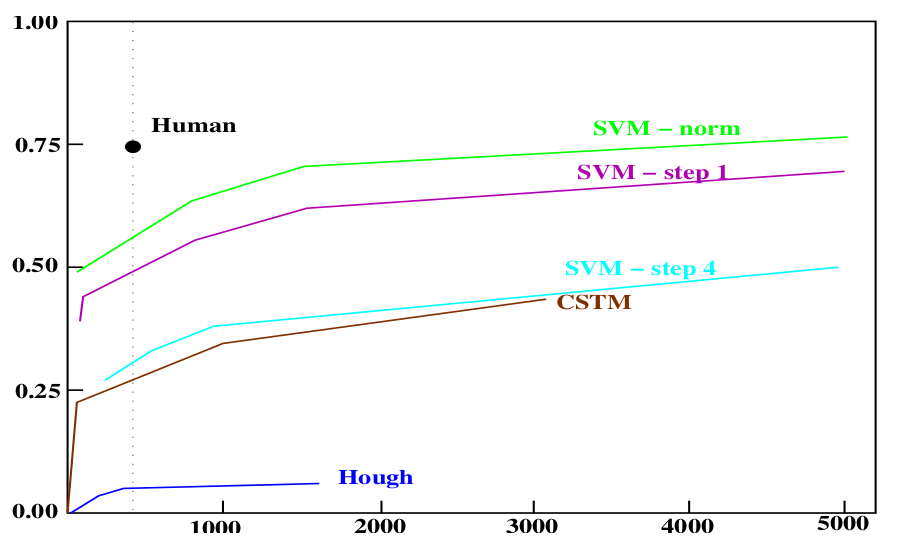
\includegraphics[width=.6\textwidth]{files/literature/roc_wetzler.png}
%	\caption{ROC performance of CSTM, SVM and Hough methods. Hough with lowest performance among all other methods \cite{wetzler2005learning}.}
%	\label{roc,wetzler}
%\end{figure}

Impact craters remains some of the most studied features in lunar and planetary science. This lead to development of Crater Detection Algorithms (CDAs) based on inspiration from pattern recognition methods. CDAs are an important subject of scientific research, as evident form the amount of publications regarding crater detection in the past. This research range from dating of planetary surfaces, searching of still unknown crater impacts on surface of the Earth and safe landing sites on other planets and asteroids. A notable application of CDAs was introduced by \cite{salamuniccar2010method} which was based on edge detection and elevation data. The CDA presented was an improvement to previous CDAs and the purpose was to contribute to Martian crater catalog. With each new planetary and lunar mission, the volume of data increases significantly. This justifies research on automatic feature detection methods and importance of their role in processing, archiving, retrieving and interpreting large amounts of image data. \cite{salamuniccar2010method} provided an overview of 73 CDA-related publications from numerous authors. Working on CDAs has been a challenging task for many reasons, e.g. multiple possible applications of CDA could provide a good solution for one specific problem on the particular planetary surface i.e. dating \cite{sawabe_2006} but not necessarily good for other surfaces depending on the terrain features or problems such as autonomous landing on other planets or asteroids \cite{leroy2001crater}. Another challenge of CDA is to distinguish between crater and non-crater objects. Set of features that separates these two, depends on the type of surface, properties of illumination and the shapes and sizes of craters. Existing algorithms mainly focus on large craters (diameter of few kilometers) located on simple surfaces which dictates a specific choice of image features \cite{bandeira2010automatic}. Therefore, it is not surprising that still no CDA available is robust as scientific community would like and that fits several research groups. Also CDA not only detects craters but also finds crater candidates that needs to be manually rejected, or corrected with diameter by computer-assistance. 

Despite of extensive research in CDAs, no algorithm became a standard tool for planetary science practitioners and crater counts continued to be done via visual inspection even as high resolution datasets keep on increasing \cite{bandeira2010automatic}. Crater appearance in an optical image depends on their level of degradation, inter morphologies (such as presence of central peaks, central pits, peak rings and wall terraces etc.), amount of overlap on other craters, quality of image (which includes illumination angle and surface properties) and on size that might differ by the order of magnitude. A notable advancement in CDA was proposed by \cite{bandeira2010automatic} which used the approach of applying series of filters for background noise removal and creates a set of features that look for the characteristics of crescent-shaped shadow of a crater. In addition to noise removal, texture recognition was added to improve algorithm precision.

Another approach begins with template matching in which image array pixels are rotated, translated or transformed to match pieces of an image. This establishes an image-based paradigm which can be extended to matched spatial features, principle components methods and artificial neural networks \cite{brunelli1993face}. An image matching algorithm known as The Continuously Scalable Template Matching (CSTM) was implemented and tested by \cite{burl2001automated} on selected lunar images. The algorithm uses templates provided by scientists for generation of a model to detect the target in a user specified continuous range of scales. Statistical efficiency of implementation of algorithm was measured on regions of the lunar maria (images provided by Clementine), which was about 80\% with 12\% false detection rate. Craters less than 5 pixels were neglected. However, the reduction in performance was caused by complexity in background terrain for crater detection on the surface of Europa (moon of Jupiter).

For crater detection automation, large focus remained on looking for circular or elliptical shape of edges on crater boundary i.e. Hough Transform \cite{honda2000crater}.  Boundary based approaches seemed to perform well (relative to image resolution) under certain conditions such as detection of the medium to large craters with limited texture in background. However the performance of these approaches deteriorated with complexity in background terrain or when craters are small. Alternating to boundary based detection methods \cite{wetzler2005learning} proposed to look directly at the pixel-level pattern in an image. The idea was to automate crater detection process by looking for adjacent bright-dark regions of proper relative size.

Most of the craters are formed as the result of meteoroid impacts. \cite{sawabe_2006} proposed an algorithm that did not depend on cameras, spatial resolution or sun illumination. It also did not require to tune any parameters either. This algorithm was improvement to their own previously proposed algorithm. Their previous method did not include pyramid representation of the image which was included in later method and thus improving accuracy and reducing processing time. The algorithm was applied on images acquired by Clementine and Apollo under different solar elevation. This approach was able to detect craters with diameter larger than \SI{240}{m}. Accuracy rate was validated by comparing with crater count results of \cite{neukum1975cratering} which was 80\% extraction of craters with multiple interpreters \cite{sawabe_2006}. 

Changeability in appearance of craters and surrounding terrain makes imaging based autonomous crater detection difficult to be applied. By experimentation it is proven that unsupervised machine learning methods work well with relatively large craters having clear edge information but their efficiency declines with increase in terrain complexity \cite{meng2009method}. In 2009 \cite{martins2009crater} performed Viola and Jones (2004) algorithm on Mars dataset gathered by the Mars Orbiter Camera onboard Mars Global Surveyor probe. In this paper author claims that no such method existed that is satisfactory for craters detection. Using this approach craters with diameter larger than 7 pixels were detected. Images of 240m/pixel were used as a data set, hence craters larger than \SI{1680}{m} of diameter were detected. The source of images used are taken from Mars orbiter camera.

An automated system for cataloging impact craters was presented by \cite{stepinski2009machine}. The system used DEM of Mars. The process of crater identification consists of two steps, in first step it identifies round and symmetric topographic depressions as crater candidate and second step identifies crater using a machine learning method. This process is AutoCrad system and applicable to any surface represented by a DEM \cite{stepinski2009machine}. A CDA was presented by \cite{salamuniccar2010method} which was based on fuzzy edge detectors and it takes input as digital topography data instead of image data. This algorithm claimed to have more correct detections compared to previous CDAs. There were also false positives which were removed manually. The data was taken from Mars Orbiter Laser Altimeter. Most of the work in automating crater detection was performed on DEMs.

\subsection{Crater Detection via Deep Learning}
Existing approaches to detection techniques can be divided into two categories: supervised (requiring a labeled input data) and unsupervised (fully autonomous). \cite{stepinski2009machine} has discussed both of these approaches and their usage. Unsupervised techniques are based on pattern recognition approaches to identify crater rims in an image as circular objects. Supervised techniques are the machine learning methods to train a classifier which is then used to distinguish between craters and the other objects. However, in both approaches features are detected by narrowing down to the set of potential candidates. In a supervised method the narrowing is achieved by thresholding a probability of positive detection by a classifier. In an unsupervised approach narrowing is achieved by thresholding a parameter that measure how well the object fits a circle. In general unsupervised approaches tend to be fast and more appropriate for detection of crater with diameter of few kilometers with no worn out edges; however their performance reduces when dealing challenging terrains and smaller sub-kilometer sized craters. This makes unsupervised not a general purpose crater detection technique \cite{emami2015automatic}. On the other hand, supervised approaches are more robust but usually slower and requires labeled input data, the performance depends on the quality and number of labeled data samples.

In 2015, a CDA was proposed by \cite{emami2015automatic} which took into account the optical images and the algorithm worked by employing a multi-scale candidate region detection step which was based on convexity cues and candidate region was verified via machine learning. In this paper a CNN classifier was tested against SVM and it was concluded that CNN classifier outperforms SVM both in terms of recall and precision \cite{emami2015automatic}. The data used for both training and testing was partially labeled by NASA scientists. Each image consists of 600x400 pixels and taken from LRO. The result of their experiment is shown in Fig. \ref{cnn_class}.

\begin{figure}[ht!]
	\centering
	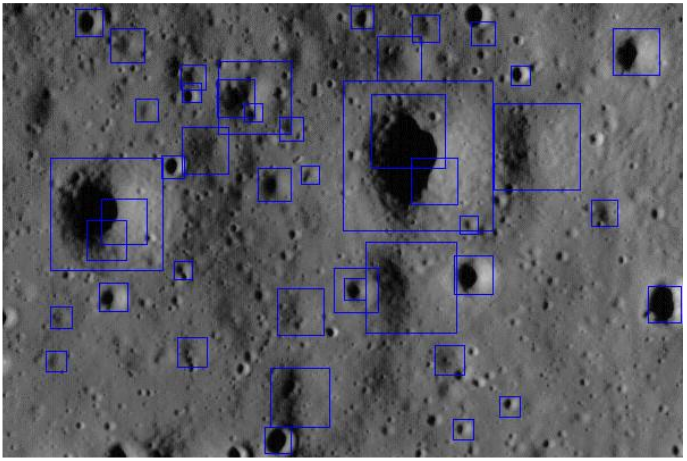
\includegraphics[width=.6\textwidth]{files/literature/emami.png}
	\caption{Verified regions in boxes on a test image \cite{wetzler2005learning}.}
	\label{cnn_class}
\end{figure}

According to \cite{palafox2017automated}, Mars Reconnaissance Orbiter opened another frontier to automate landforms detection process. Authors came up with two different approaches. These are detection of volcanic rootless cones and transverse aeolian ridges using CNNs and also using SVM with HOG features. They showed that CNNs can detect a wide range of landforms and has a better accuracy and recall than traditional classifiers based on SVMs. \cite{wang2018crateridnet} presented a method composed of CNN architecture and named it as CraterIDNet which takes remotely sensed planetary images as input and outputs detected craters, their apparent diameters and their positions. The experiments shows that CNN based architecture has the advantages of high robustness, detection and identification accuracy over other methods used by \cite{urbach2009automatic}, \cite{bandeira2010automatic} and \cite{ding2011subkilometer}.

A deep learning model based on CNN architecture was introduced by \cite{silburt2019lunar} for crater identification on lunar DEMs. The author also applied transfer learning to craters on Mercury. In this paper random DEMs from LRO and Kaguya were taken as an input data. Thus it was a global gray scale map. The proposed CNN detects only half of the caters per target. The post-CNN recall is lower at 57\% $\pm$ 20\%. Detections for craters less than 15 pixels of diameter largely improved the post-CNN test recall to $83 \% \pm 16 \%$. The sample of DEM from \cite{silburt2019lunar} is shown in Fig. \ref{dem_}.

\begin{figure}[ht!]
	\centering
	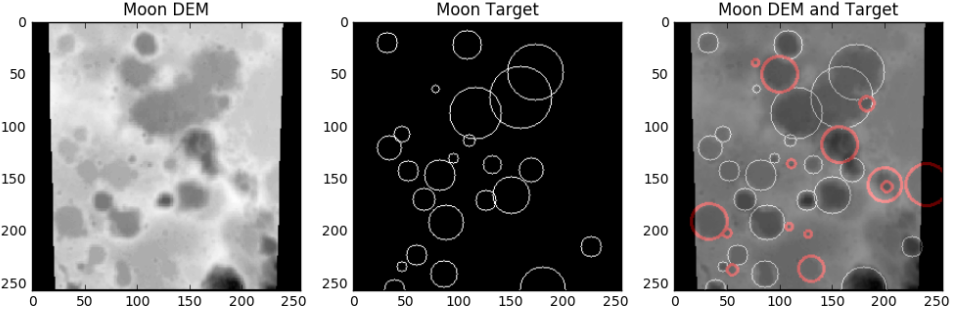
\includegraphics[width=.8\linewidth]{files/unet/dem.png}
	\caption{Left is the Moon DEM sample and middle image shows prediction of craters and right one shows the missing classifications which are marked in red circles \cite{silburt2019lunar}.}
	\label{dem_}
\end{figure}

\cite{cohen2016crater} demonstrated that ConvNet for crater detection outperformed previously tested methods including CDAs presented by \cite{stepinski2009machine}, \cite{bandeira2010automatic} and \cite{ding2011subkilometer} on the same dataset. An algorithm based on Fast-RCNN was proposed by \cite{emami2015automatic} for lunar crater detection on LRO dataset and it showed great potential in CNN applications for this task. ConvNets are becoming more common in crater detection problems and these are specially of more importance because of the fact that major part of CDAs is not accepted by planetary science community as general purpose crater detection tools \cite{emami2015automatic}. Intersection over Union (IoU) was taken as 30\% by the author based on experimentation of precision and recall values.

\begin{figure}[H]
	\centering
	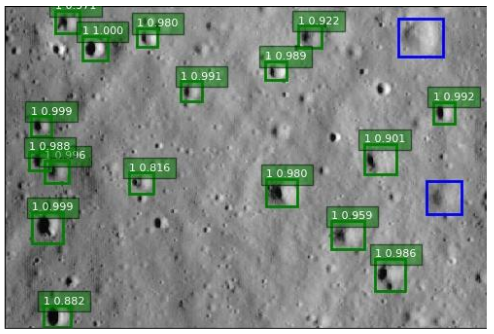
\includegraphics[width=.6\linewidth]{files/literature/fastrcnn.png}
	\caption{Crater detection results on LRO dataset by using Fast R-CNN based network. Blue squares represent missing craters by the author \cite{emami2015automatic}.}
	\label{dem}
\end{figure}

Recently \cite{ali2019automated} experimented with instance segmentation method on crater detection problem. The algorithm is well known Mask-RCNN presented by \cite{he2017mask}. Model was trained on lunar DEMs to detect craters in an image and simultaneously producing a mask for each crater that also traces the outer rim of it. Then a post-processing pipeline was introduced to find the closest fitting ellipse to these masks. However, optical images were not taken into account because the target diameter was $\geq$ \SI{5}{km} which justifies the use of DEMs.

\begin{comment}
\cite{honda2000crater} compared multiple methods for crater detection and categorization. Those included combinational Hough transform and genetic algorithms. The idea was to first detect then classify according to shape of craters i.e. cone-shaped, bowl-shaped or flat-floored with central peak.
\end{comment}


\begin{comment}
CNN models composed of multiple processing layers learn the representation of data with numerous levels of abstraction by deep learning. These methods have made dramatic improvement in state of the art visual object recognition, speech recognition, object detection and many other areas such as genomics and drug discovery. Deep learning uses backpropagation algorithm to indicate how a machine should change its internal parameters of each layer from representation in the previous layer. This allows learning of machine to correctly represent i.e. patterns in an input.

Deep learning methods are the representations of multiple levels obtained by composing non linear modules such that each module transform the representation from one level to a higher level making it more abstract. Composition of such transformations makes it possible to learn complex functions. For classification, it is performed in different layers. The image is in the form of an array of pixel values, typically the first layer represents presence or absence of edges on specific locations in image.  The second layer detects a shape by visualizing edges. The third layer may densify the shape into more prominent features and later layers make use of these computations to detect objects as a resultant of combination of shapes.

Object detection and classification can be performed in supervised machine learning. In a typical supervised machine learning method a system is built that can classify different objects (belonging to several classes such as human, animals, trees, cars and bikes etc.) then first it is required to have a labeled data set of such objects. For example to categorize horses and people, it is needed to have a data set which will consist of labeled images containing horses and people. This dataset would be required to train the machine about learning that how horses and people looks like so that it can classify the categories. The algorithm then outputs a vector of scores for each category. To get the category rightly identified, it is required to have the highest score for desired category out of all categories. This is not likely to happen without training of the algorithm. It is needed to compute a loss function that calculates the distance or error between the output scores and desired pattern of scores. This function helps algorithm to adjust its internal parameters that could be changed to reduce this error. These parameters are commonly referred to as weights and are real numbers.
\end{comment}

\begin{comment}
\subsection{Bounding Box Proposal}
In object detection, a bounding box (also referred to as region of interest or box proposal) shows the existence of object. It is a rectangular region of the input image containing the object. Bounding boxes can be generated by some heuristic search methods such as finding region proposal by objectness, region proposal network (RPN) or by selective search method. A bounding box can be either represented by storing its two corner coordinates $(x_0, y_0, x_1, y_1 )$  or most commonly by storing its center location along  with width and height such $(x, y, w, h)$. A bounding box is generated on the basis of confidence score that how likely an object exists inside the box. The difference between two bounding boxes is usually measured as the L2 distance of their vector representations. Another simplest way is to compare the images by taking pixelwise difference and summing up all the differences. To perform such procedure, given two images can be represented as vectors $I_1, I_2$ then L1 can be computed as:

\begin{align*}
d_1 (I_1, I_2) = \sum_{p} \left| I^p_1 - I^p_2 \right|
\end{align*}

\begin{figure}[ht!]
\centering
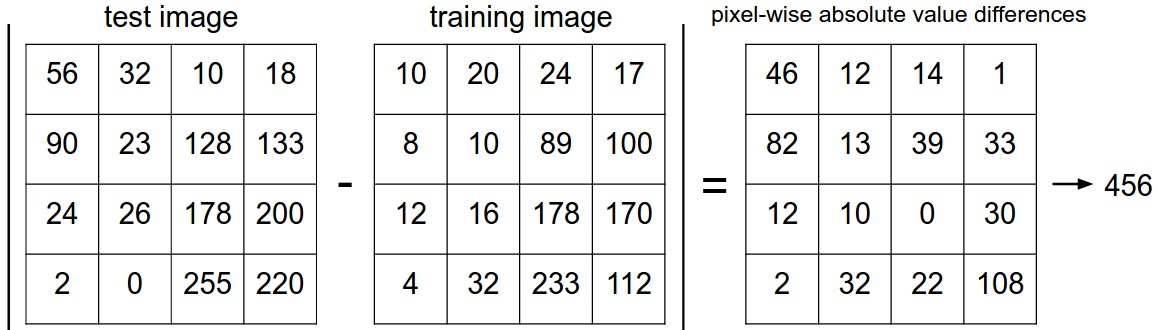
\includegraphics[width=.6\linewidth]{files/nneg.jpeg}
\caption{Example of two images which are represented as vectors and pixelwise difference is calculated to compare both images with L1 distance. This example shows one color channel. All the pixel-wise differences are added to denote a single digit value. If this value is close to zero then it indicates that images are identical. A large value shows that both images are very different.}
\label{fig: bbp.}
\end{figure}

The difference between bounding boxes can also be measured by the L2 distance. Similar like L1, images are represented in a vector form. $w$ and $h$ can be log-transformed before calculating distance. L2 has the geometric representation of computing euclidean distance between two vectors as:

\begin{align*}
d_2 (I_1, I_2) = \sqrt{\sum_{p} \left( I^p_1 - I^p_2 \right)^2}
\end{align*}

In simple words this operation also computes the pixelwise difference like L1 but here all the differences are squared then added and finally equation is subjected to square root. Difference in measurement between both metrics differs in a way that L2 prefers many medium disagreements to one big one when it comes to difference between vectors.

In case of multiple bounding boxes a common algorithm to merge them is non maximum suppression (NMS). A bounding box that overlaps another one having higher confidence score with a factor such as its intersection over union (IoU) is greater than IoU threshold, is removed. Intersection over union provides similarity between two bounding boxes. ${\textit{Area of Overlap}} /{\textit{Area of Union}} = IoU
$. The bounding boxes play an important role in setting up dataset for the algorithm. Learning of the algorithm largely depends on correctly placed bounding box on the object.

With sliding windows, a bounding box can be attained but it may not properly fit the object. With bounding box and stride size, it might be only able to cover a part of the object and not the complete object. This problem can be solved using an approach developed by \cite{redmon_you_2016} where a picture is divided into multiple grids and an image classification and localization algorithm is applied to each grid. Every grid has a label $y$ which represents some parameters as shown below:

$$
y =
\begin{bmatrix}
p_c\\
b_x\\
b_y\\
b_h\\
b_w\\
c_1\\
\end{bmatrix}
$$

where $p_c$ is whether or not there is an image, $b_x, b_y, b_h$ and $b_w$ is to specify bounding box, $c_1$ is object class (i.e, craters). If there is no crater then $p_c$ will be zero and hence the entire vector is to be dropped. When $p_c$ = 1, it represents there is a crater and all the bounding box parameters would specify position of this box and hence the value of $c_1$ would be 1. Each grid cell will have this output vector $y$. The idea is to feed an input image and run forward pass (convolution, max pooling and relu) to get this output vector $y$.

The evaluation of object detection algorithm can be performed using $IoU$. As mentioned before, it gives the ratio between area of overlap and area of union. So if the algorithm outputs a bounding box which does not properly fit the ground truth bounding box representing the object then by convention the answer is taken correct if $IoU \geq 0.5$. If predicted and ground truth bounding boxes overlaps perfectly then IoU would be 1. The higher the IoU, the more accurate the bounding box is.

\end{comment}

\begin{comment}
\subsection{Linear Classification}
It is one of the simplest technique to classify an object. Eventually it is extended to the entire Convolutional neural network. It has two major components. One is score function which does the mapping of raw data to the class scores and other one is a loss function that defines how different predicted score is from the ground truth labels. Typically loss function is higher initially and thus required to be minimized with respect to the score function parameters. This minimization is also referred to as optimization. 

To define a score function which is the first component of linear classification, it is required to have information about number of images $\boldsymbol{N}$ with dimension  $\boldsymbol{D}$ i.e. the size of image (pixels and channels) and distinct categories $\boldsymbol{K}$ which are the number of classes. A simplest possible function for linear mapping:

$$
f(x_i, W, b) = Wx_i + b
$$

Here $x_i$ is the image which is flattened out to a single column vector of shape $[D \times 1]$. $\boldsymbol{W}$ is of size  $[K \times D]$ and is often referred to as weights, whereas $b$ is called bias vector with size  $[K \times 1]$. Multiplication of matrices $Wx_i$ gives separate classifiers in parallel where each classifier represents a row of weight matrix. The goal is to set the weights and bias parameters in a way that the output score match the ground truth labels of training data set as such that the correct classes has higher score than the incorrect classes.

A linear classifier computes the score of a class by taking weighted sum of all pixel values in all the channels of an image. If there is an image of ship then most likely surrounding pixels of ship would be blue (because of water presence). That means across blue channel weights will be largely positive whereas mostly negative in other channels i.e. red and green. Positive weights in blue channel increases score of ship class.
\end{comment}

\begin{comment}
\begin{figure}[H]
	\centering
	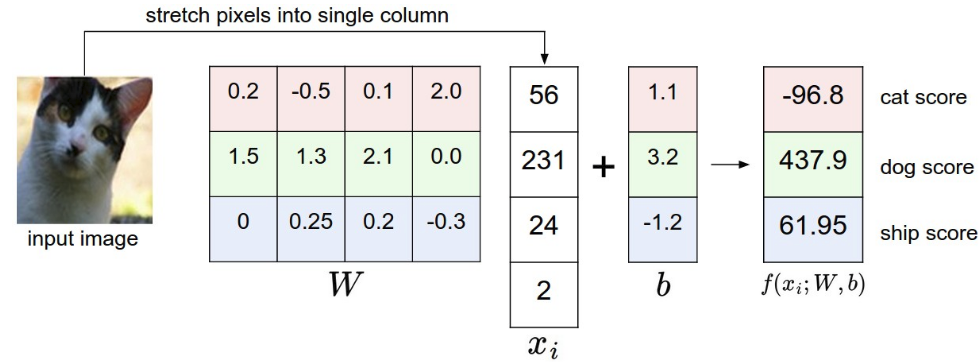
\includegraphics[width=90mm,height=33mm,  scale=0.8]{files/cnn_architecture/linear_class.png}
	\caption{The graphical representation of eq 
		($f(x_i, W, b) = Wx_i + b$). It shows that an image $x_i$ is represented as a one dimensional vector which is multiplied by set weights and resultant is added with a bias leading to the highest score for detection of cat image. The weights are set badly as classifier thinks it is a dog instead of a cat.}
	\label{fig: linear classifier}
\end{figure}
\end{comment}

\begin{comment}
\subsection{Weights Initialization}
Initially weights of a CNN before training are randomly chosen. The key rule to pick a random weight is not to initialize with a too large or too small value to avoid the well known problem of vanishing or exploding gradients. Some initialization methods like He Initialization and Xavier Initialization are the common practices to setup weights. Before training, the CNN is not able to make meaningful predictions because there is no relation between the input images and their annotated outputs with classes. This process is performed in training where weights are adjusted in a way so that difference between desired output and network output is minimized. In other words network is trained to look for the right features needed for classification.

\subsection{neural network Overview}
In supervised machine learning object detection task can be achieved using different approaches. There are various architectures based upon statistical functions. A neural network is made up of neurons having learnable weights and biases. It means that during training process, weights and biases can be updated. A neuron in an artificial neural network is referred to a mathematical function. It receives inputs which can also be output of neurons from a previous layer, weighs each input and sum them up. A weight shows the strength of connection of one neuron to another neuron in next layer. Every neuron has a bias and it determines if the neuron is activated or not. Biases are added to the product of weight and value of neuron. Each neuron is fully connected to all the neurons of previous layer. These neurons do not share any connection within a single layer. The last fully connected layer is referred to as "output layer". The network takes an input and computes the output by taking a dot product. The entire network takes raw image pixels and presents an output in the form of a digit representing the class score for an object. Output layer represents the class scores. It expresses a single differentiable score function. There could be few to many hidden layers and a fully connected layer that has a loss function i.e support vector machine (SVM) or softmax. A typical neural network architecture is shown below:

\begin{figure}[H]
\centering
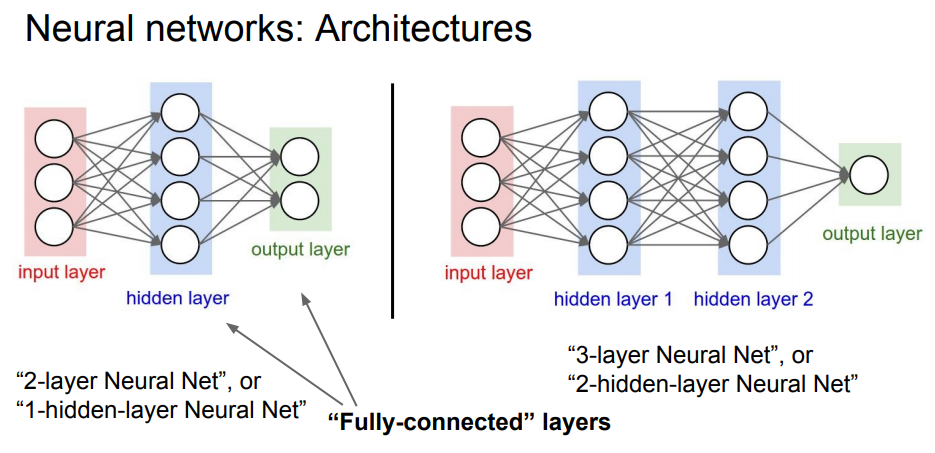
\includegraphics[width=.6\linewidth]{files/NN.jpeg}
\caption{A typical neural network architecture}
\label{fig: neural network architecture}
\end{figure}

Artificial neural networks are very similar to convNets but they do not convolute on an image through a filter thus leading to many more parameters as compared to CNN i.e. in CIFAR-10 dataset, images are of 32x32x3 (width, height, 3 color channels). That means in an input image of size 32x32x3, an Artificial neural network would have 3072 weights. These weights tend to increase with size of image.
\end{comment}

\begin{comment}
\subsection{Convolutional neural network Overview}
Just like Artificial neural networks as shown in Fig \ref{fig: neural network architecture}, convNets are also made up of neurons consisting of weights and biases which are learnable. Each neuron receives an input then performs a dot product and optionally follows it with a non-linearity. The entire network represents a single differentiable score from the raw image input to the output score. Last fully connected layer has a loss function which represents the error score. This entire process is referred to as forward pass. In convNet, the architecture assume inputs as images which provides flexibility of encoding certain properties. This greatly reduce the amount of parameters to learn and make forward pass more efficient. The layers of convNets have neurons arranged in 3 dimensions (width, height, depth). The neurons in a layer are not connected to all of the neurons in a previous layer like in an Artificial neural networks, instead they are connected to only small region of previous layer. The output results into a single vector of class scores by reducing the full image. Following are the types of layers in a Convolutional neural network:

\subsubsection{Fully Connected layer}
After multiple convolution and pooling operations, finally an output can be generated in the form of a class. Convolution and pooling layers only extract the features and reduce amount of parameters from the input images. Fully connected layer (FC layer) is applied at the end to generate the required output equal to the number of classes. There can be multiple FC layers to further minimize the amount of parameters. In convolution the resultant is generation of 3D activation maps whereas the intention is to know whether the image belongs to a particular class or not. The output layer (which generates the class scores) has a loss function and once the forward pass is completed, backpropagation begins to update biases and weights for loss and error reduction. An overview of the architecture is shown below:

\begin{figure}[H]
\centering
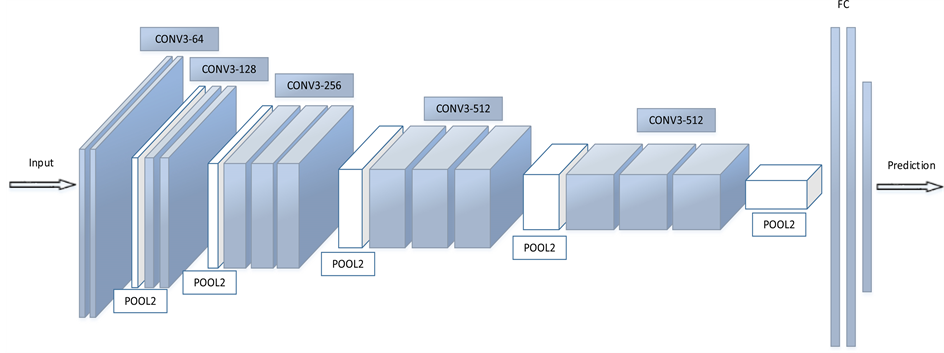
\includegraphics[width=.6\linewidth]{files/cnn_architecture/arch.png}
\caption{Convolutional neural network Architecture \cite{2016face}}
\label{fig: CNN architecture}
\end{figure}
\end{comment}

\begin{comment}
\subsubsection{Softmax Classifier}
A binary classifier is a function that determines the class of an object i.e. if there is a crater (which has an assigned class of 1), ideally it will recognize it as one. Softmax classifier is generalization of binary form of logistic regression. It interprets the scores as unnormalized log probabilities for each class and has the following form:

\begin{equation}
\label{singlesoftmax}
L_i = -\log\left(\frac{e^{f_{y_i}}}{ \sum_j e^{f_j} }\right) 
\end{equation}

Loss function has to minimize the negative log likelihood of correct class. Here $f$ is the mapping function $(x_i,W)$ and $f_j$ represents the j-th element of the class scores vector $f$. In order to represent softmax function for the entire dataset, one would need to take the mean of $L_i$ over all training data and hence softmax function is represented as:

\begin{equation}
f_j(z) = \frac{e^{z_j}}{\sum_{k=1}^{K} e^{z_k}}
\end{equation}

$z$ is the vector of score of arbitrary real values and those are squashed to a vector of values ranging between zero and one. The sum of these values is one. The form $\frac{e^{f_{y_i}}}{ \sum_j e^{f_j} }$ in eq.$\ref{singlesoftmax}$ is the estimated distribution. Plugging it into eq.$\ref{crossent}$ makes it clear that softmax is minizing the loss.
\end{comment}

%\section{Research Question}
%\begin{enumerate}
%	\item How to evaluate the performance of algorithm?
%\end{enumerate}

\subsection{Planetary Surface Age Dating}
Moon provides an ideal test site for studying crater records, particularly since almost all of the lunar endogenic activities ended more than around 3 Giga years (Ga) with some exceptions \cite{hiesinger2000ages}. Therefore, in last \SI{3}{Ga}  crater impacts have dominated to change lunar landscape. Space missions have also studied the Moon extensively and collected samples from the Moon have provided a unique opportunity to assign age to craters and areas where accumulated crater are counted \cite{stoffler2001stratigraphy}. Therefore, on the Moon it can be estimated that cratering rate is the number of craters of a given diameter that are accumulated at given surface during a given time interval.

CSFD reflects the standard distribution of crater impacts. By plotting CSFD against diameter, the age can be estimated by the help of lunar production functions. These well known methods are proposed by W. Hartmann and G. Neukum.

\subsubsection{Hartmann Production Function (HPF)}
Hartmann uses a log-incremental SFD representation with a standard bin size for diameter to represent the CSFD of terrestrial planets. The obtained results are referred as Hartmann production function or HPF. The number of craters per kilometers squared are calculated for a certain diameter range which is $D_{L} < D < D_{R}$, this range represents a bin where $D_{L}$ and $D_{R}$ are the left and right boundaries of diameter range respectively. The standard bin width is $D_{R}/D_{L} = 2^{1/2}$. Findings from most of the lunar mare basalt samples suggests a narrow range of ages between 3.2 to \SI{3.5}{Ga} \cite{stoffler2001stratigraphy}. However, lunar production functions takes into account that crater populations are not effected by any processes. Therefore, if such processes have occurred that changed crater formations then age estimation will be different than the actual. In case of lunar surface, some lava flows on the surface could be younger \cite{hiesinger2000ages} therefore the age variation is represented by a factor of 1.1.

The tabulated HPF is considered reliable for the projectile of a production function because the crater counts from different areas of the Moon are combined and averaged. The incremental form of HPF takes form of a piece-wise three segment power law \cite{ivanov2002comparison}.

\begin{equation}
\log N_{2^{1/2}} = -2.616 - 3.82 \log D_{L}, (D<1.41km)
\end{equation}

\begin{equation}
\log N_{2^{1/2}} = -2.920 - 1.80 \log D_{L},
(1.41km < D < 64km)
\end{equation}

\begin{equation}
\log N_{2^{1/2}} = -2.616 - 3.82 \log D_{L},
(D>64km)
\end{equation}

The function is represented in Fig. \ref{HPF}. Hartmann chose power law segments in 1960s when this work started. Some of the selections were on the basis of historical reasoning that only the craters branch with diameter range between \SI{1.41}{km} and \SI{64}{km} was well established. At that time there were already existing laws of meteoroids and asteroids and Hartmann's attempt was to relate those laws to lunar data.


\subsubsection{Neukum Production Function (NPF)}
Neukum proposed an analytical function describing the CSFD of lunar impact craters. He wrote a series of publications in description of his function. For summaries, see \cite{neukum1994crater} and \cite{neukum1983meteoritenbombardement}. Neukum showed that the production function is stable since \SI{4}{Ga}. The time Neukum proposed this function, a full size crater spectrum was known. His approach was different from Hartmann in a way that he computed a polynomial fit to the cumulative number of craters. Where as Hartmann proposed a piece-wise exponential equations for his production function. For the time period of \SI{1}{Ga}, Neukum's production function can be represented as:

\begin{equation}
\log_{10} (N) = a_0 + \sum_{n=1}^{11} a_n[\log_{10} (D)]^n.
\end{equation}

In above equation D is in km, N is the number of craters with diameters greater than D per squared kilometers per Ga and values of coefficients $a_n$ are provided in table. The above equation is valid for crater diameters from \SI{0.01}{km} to \SI{300}{km}.

On the basis of age assumption NPF was fit to the crater count. It is notable that both HPF and NPF are a good match for the crater diameter data under \SI{1}{km} range. However, with D $>$ \SI{1}{km}, HPF has higher values than NPF and both functions meet again at diameter of approx. \SI{40}{km}. In Fig. \ref{HPF} it can be seen that the maximum variation between the two functions is of the factor 3 around the diameter of approx. \SI{6}{km}. Note that below the diameter of \SI{1}{km} and between 30-\SI{100}{km}, both of the functions are same. After \SI{100}{km} both started to decline but HPF declines more rapid as compared to NPF.

\begin{figure}[H]
	\centering
	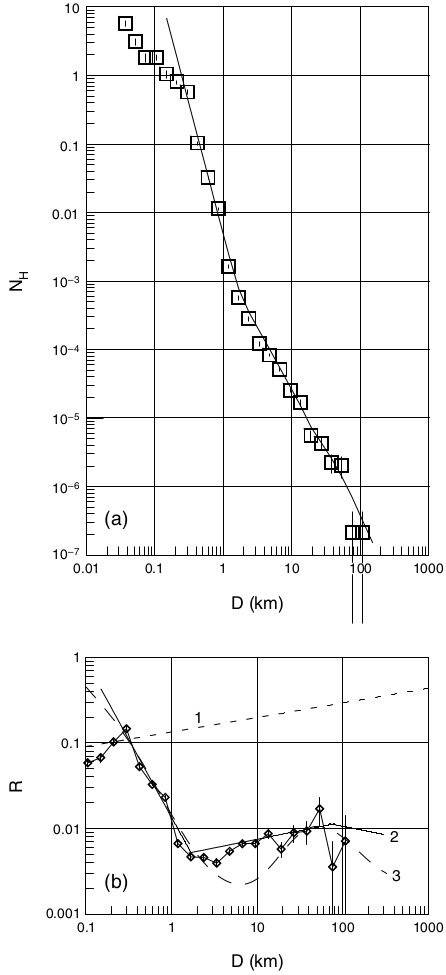
\includegraphics[width=75mm,height=170mm,  scale=0.8]{files/lunar_functions/HPF.jpg}
	\caption{These plots are taken from \cite{ivanov2002comparison}. It shows the representation of the Hartmann production function (HPF). HPF is a function composed of set of
		points shown in the plot. Straight lines represent the piece-wise
		power law fitting to the data (equation (15)). Lower figure shows the comparison of Neukum (NPF) and Hartmann (HPF)
		in the R plot representation. The maximum discrepancy between
		HPF (2) and NPF (3) (roughly a factor of 3) is observed in the
		diameter bins around D close to \SI{6}{km}. D less than \SI{1}{km} and diameter range between 30-\SI{100}{km}, both production functions outputs similar results. The dashed line 1 represents the approximate saturation level estimated by Hartmann (1995).}
	\label{HPF}
\end{figure}

%The idea of machine learning existed well before early 2000s but because of lack of powerful GPU it was not possible to process the intense computation. In last decade, object detection techniques have been improved considerably. In 2013 a method was developed that refined the object detection performance from previously used approaches. The idea was to combine region proposals with CNN's and the method was referred to as R-CNN \cite{girshick_rich_2013}. Since then pixel level processing advancement in the algorithm has been made and in 2017 a team of Facebook researchers came up with a new algorithm that contributed to reduced processing time and increased accuracy (up to 99\%) \cite{he_mask_2017}. They came up with a method that does not only detect an object but also generates a high quality segmentation mask for each instance \cite{he_mask_2017}.


%YOLO (You Look Only Once) is another method which was developed with an intention to detect objects at a greater speed than existing algorithms. YOLO lacks state of the art object detection accuracy achieved by other CNN algorithms i.e. Faster R-CNN and Mask R-CNN. But as it states you look only once, YOLO detects an object very quickly as compared to Mask R-CNN but it struggles to localize some objects, specially small ones ~\cite{redmon_you_2016}. This is because of its spatial constraints on bounding box predictions as every grid cell can have only one class.

%\subsection{Dataset}
%For training and testing of model. The dataset is taken in the form of images from LRO in 2 different formats: grayscale and RGB. These images are of moon and consists craters of different sizes.

\section{Methods}
With multiple lunar missions there are millions of images taken by various satellites which are important source of data for crater detection. Deep learning methods require labeled input data for training so that an algorithm is able to detect objects. Performance of these algorithms increases with increase in training samples. According to size and distribution of lunar craters there can be thousands of them in one NAC image of LRO which represents the area of \SI{266}{km}². Generating a large labeled or groundtruth data set is expensive even though a domain expert is not necessarily required for image annotation. Deep neural networks typically require thousands of images for training such as Mask-RCNN. Often transfer learning is also helpful for loss convergence when training on a new data set. On the other hand, there are deep learning models that have proven to perform well on small data set with only few hundred images. These shallow networks can also be trained from scratch on a data set.

Below are the methods that were applied in an attempt to detect lunar craters on part of one of the NAC images. 

\subsection{Semantic Segmentation}
Image level classification means treating each image as an identical category. In object detection an object is localized and recognized with respect to type of its class. Whereas semantic segmentation is also called pixel-level classification. This is a task of clustering parts of an image together which belong to the same object class \cite{thoma2016survey}. It can also be treated as pixel-level prediction because it classifies each pixel of an object into its category. However, this type of segmentation does not distinguish between different instances of an object.

\subsection{Hough Circle Transformation}
Hough proposed a procedure for line detection in images. This method was extended to GHT for detection of curves in a picture and detailed procedure is provided by \cite{duda1972use}. This has remained one of the widely used methods for circle detection in the field of computer vision.

\subsection{Instance Segmentation}
Instance segmentation provides not only a pixel-level segmentation to an object but also determines the different instances of objects in an image. This addition makes instance segmentation more challenging that semantic segmentation. In last 3 years neural networks have been introduced that are able to perform instance segmentation and also keep better accuracy as compared to state of the art methods. But a successful training of such deep networks requires many thousands of labeled samples. 

In this thesis, the proposed method for crater detection with a small dataset is based on an encoder-decoder architecture. This architecture is a slight variation of a neural network also known as U-Net presented by \cite{ronneberger2015u}. This network is chosen to perform pixel-wise segmentation because of three main reasons; it does not require several thousands of images for training, it does not need transfer learning and can be trained from scratch which makes it robust, it also has a simple network structure which can be easily altered to fit segmentation goals. U-Net has also proven to be an effective network for segmenting single class in satellite data \cite{Snuverink2017}. U-Net was originally developed for segmentation of biomedical images and it achieved an average IoU of 77.5\% on DIC-HeLa dataset in ISBI cell tracking challenge 2015 which was the best score at that time. A different version of U-Net was applied for Martian craters segmentation by \cite{delatte2019segmentation} and 76\% accuracy was achieved along with age dating results consistent with human annotations for same geological units. This application demonstrated that CNN offers an advantageous approach to labor-intensive challenging task of satellites image analysis. 

\subsection{Contrast Limited Adaptive Histogram Equalization (CLAHE)}
Histogram equilization considers the global contrast of an image. Therefore in cases where image has high pixel values, such regions tend to loose alot of information as those pixels are stretched further towards 255 and object becomes too bright. 

By using CLAHE, the image is divided into small blocks also called tiles (function implemented in OpenCV has default tile size of 8x8). Then each one of these tiles histogram equalized. This makes histogram confined to a small area. It will be amplified if noise is there. Contrast limiting is applied to avoid this problem. The default contrast limit is 40 in OpenCV and pixels with larger values are clipped and distributed to other bins uniformly before application of histogram equilization. After that there are artifacts in tile boarders which are removed by the application of bilinear interpolation. By applying CLAHE the detection of craters increased up to 40\%. 

\begin{figure*}[ht!]
	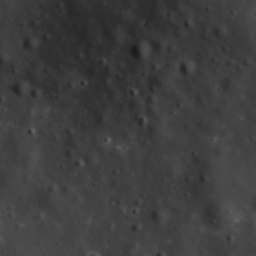
\includegraphics[width=.4\textwidth]{files/unet/IMG-0.png}
	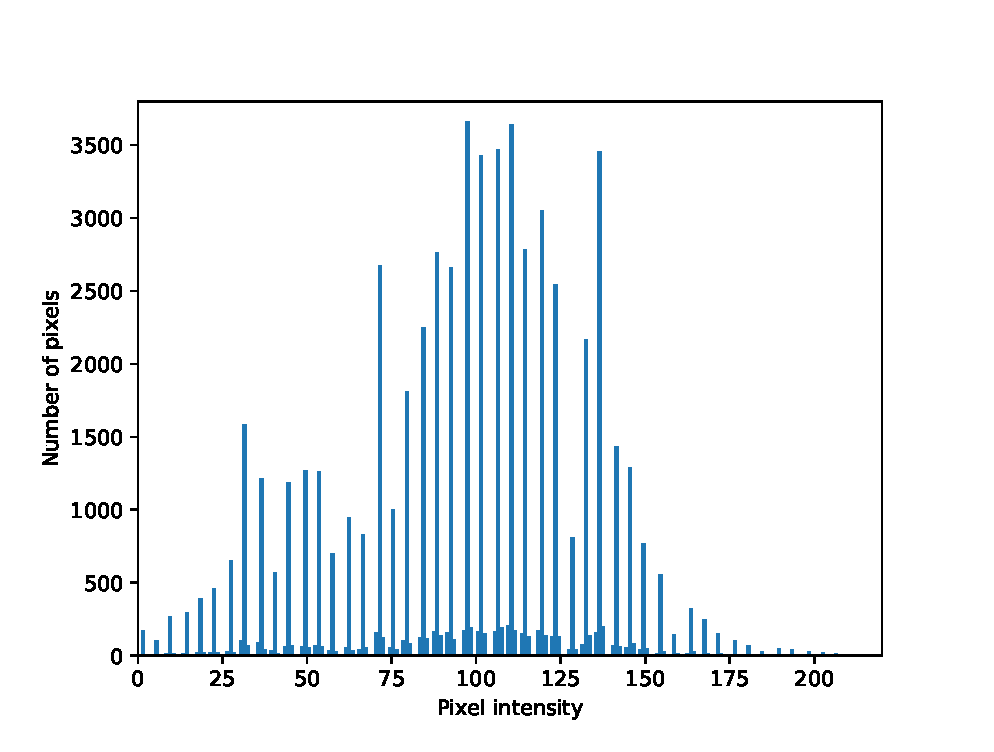
\includegraphics[width=.6\textwidth]{files/unet/0_hist.eps}
	\caption{Histogram of an image before contrast limited adaptive histogram equilization}
	\label{hist}
	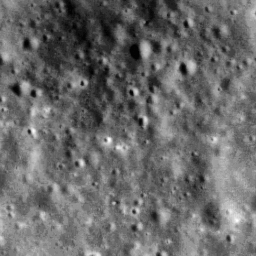
\includegraphics[width=.4\textwidth]{files/unet/0_clahe.png}
	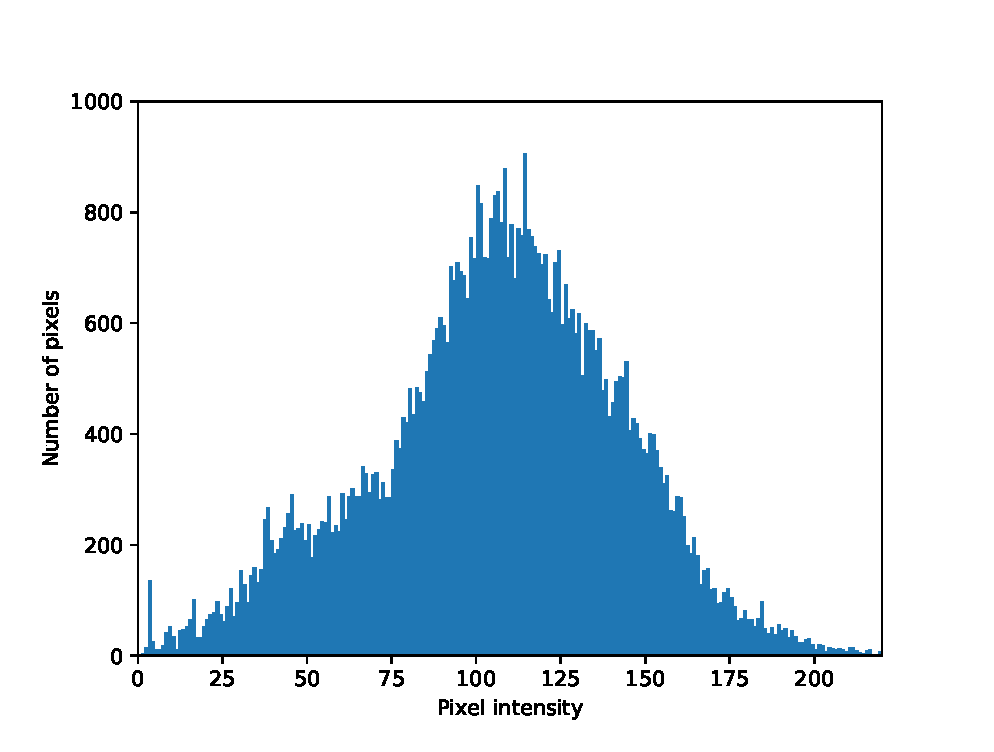
\includegraphics[width=.6\textwidth]{files/unet/0_hist_clahe.eps}
	\caption{Histogram of an image after contrast limited adaptive histogram equilization}
	\label{clahe}
\end{figure*}

\subsection{Binarization Methods}
Several binarization methods are applied to experiment best suited thresholding for probability maps. These methods are discussed below.

\subsubsection{Otsu's Method}
This method was presented by Scholar Otsu. It is widely used till today because of its simplicity and effectiveness. Otsu's method determines a threshold value automatically. In lunar images probability map, the histogram has two peaks. Otsu in simple words take the approximate middle value of the two peaks. This is unlike a global thresholding where an arbitrary value is normally chosen. This method works on the principle of minimizing the intra-class variance, defined as weighted sum of variances of two classes. Given in Figure: \ref{otsu thresholding} is the outcome of this method.

\begin{equation}
\sigma_{w}^{2}(t)=\omega_{0}(t) \sigma_{0}^{2}(t)+\omega_{1}(t) \sigma_{1}^{2}(t)
\end{equation}

Here $\omega_{0}$ and $\omega_{1}$ are the probabilities of two classes which are separated by a threshold $t$. $\sigma_{0}^{2}$ and $\sigma_{1}^{2}$ represents the variances of two classes.

\subsubsection{Sauvola's Algorithm}
It takes graysscale images as input. If an image has three color channels then its necessary to convert that into grayscale image. Savoula proposed to compute a threshold of a grayscale image at each pixel using:

\begin{equation}
T=m \times\left[1+k \times\left(\frac{s}{R}-1\right)\right]
\end{equation}

Here $k$ is user defined parameter, $m$ is mean and $s$ is the local standard deviation computed in a certain window size which is centered on current pixel and $R$ is the dynamic range of standard deviation. $R$ = 128 with 8-bit gray scale images. Window size for computation of $m$ and $s$ is user defined. This method is computationally efficient and relatively works well on noisy and blurred documents \cite{szegedy_going_2015}. This method performs over-segmentation which can be visualized in Figure: \ref{sauvola thresholding}.

\subsubsection{Niblack Method}
This method was proposed in 1986 by Niblack. Before introduction to this algorithm, global methods were used for image segmentation which are not capable to preserve the minute details of an image during segmentatio. Therefore this method was developed to preserve minute details at local while object separation. A new concept of local window was introduced. Niblack computes the threshold by calculating local mean and standard deviation of pixels value in a local window confined to an image. The equation is given as:

\begin{equation}
T_{d}=m(x, y)+k \times s(x, y)
\end{equation}
where $m(x, y)$ is local mean and $s(x, y)$ is standard deviation and $k$ is an image dependent parameter selected manually by the user (normally -0.2 for dark foreground and +0.2 for dark background). The resulting segmentation is not very different from Sauvola's method as can be viewed in Figure: \ref{Niblack_th}.

\subsubsection{Adaptive Mean Thresholding}
In this type of thresholding, algorithm computes the threshold for a pixel on the basis of a small region around it. This results into various thresholds for different regions of the same image. This gives better results for images which are illumination variant. Outcome of this method is given in Figure: \ref{Adaptive mean thresholding}.

\subsubsection{Mean Thresholding}
This threshold is simply mean of the grayscale values of an image. All the values higher than this mean (which is a float number) are considered to be foreground and rest is background. Output of this method can be seen in Figure: \ref{mean_th}.

\subsubsection{Yen Thresholding}
This threshold method takes number of bins used to calculate histogram and returns a threshold based on maximum correlation criterion. It was proposed by \cite{yen1995new}. Result can be seen in Figure: \ref{Yen thresholding}.

\subsubsection{Li Thresholding}
This method is based on minimum cross entropy. The idea is to select a threshold that minimizes cross entropy between thresholded and original image. It was presented by \cite{li1993minimum}. Thresholding result is shown in Figure: \ref{Li thresholding}.

\subsubsection{Isodata Thresholding}
Histogram based threshold alo known as inter-means or Ridler-Calvard method. Threshold is computed by separating the image into two groups of pixels. The resultant threshold lies in the midway between mean intensities of these two groups. That is average of the two. It was proposed by \cite{ridler1978picture}. Figure: \ref{isodata thresholding} shows the outcome of this method.

\subsection{Evaluation Method}
Precision, recall and F1-score evaluate the performance of algorithm. Precision is defined as the percentage of results which are relevant and mathematically written as:

\begin{equation*}
\text{Precision} = \frac{\text{True positive}}{\text{True positive + False positive}}
\end{equation*}

True positives are correctly identified craters and false positives are craters detected by the algorithm but no crater exists on that location.

Recall is defined as the percentage of total relevant results correctly classified by the algorithm and is given by:

\begin{equation*}
\text{Recall} = \frac{\text{True positive}}{\text{True positive + False negative}}
\end{equation*}

In the above equation false negatives are simply missed craters by the algorithms. For overall evaluation both of these metrics are taken into account and finally F1-score has been computed by the given equation:

\begin{equation*}
\text{F1-score} =2 * \frac{\text { Precision } * \text { Recall }}{\text { Precision }+\text { Recall }}
\end{equation*}

Hence higher the F1-score better is the performance of algorithm and vice versa. Following the experiments of \cite{emami2015automatic} a verified region is a true positive if it has more than 40\% overlap with a ground truth crater; otherwise, it is a false positive.

\section{Model Architecture}
The model architecture is composed of contracting and expansive paths as shown in the Figure: \ref{fig:U-net}. Like in a typical CNN, the image becomes smaller as a result of convolutional operations. U-net has the same effect and thus left part of this pipeline is referred to as contracting path. It consists of several convolutional operations such that each of two unpadded convolutional layers with an activation of rectified linear unit (ReLU) are followed by a layer of max pooling of the size 2x2. This results into downsampling of the image. During each downsampling step the number feature channels are doubled as seen in the Figure: \ref{fig:U-net}. This part ends up with a dropout function before it starts expanding.

\begin{figure}[H]
	\centering
	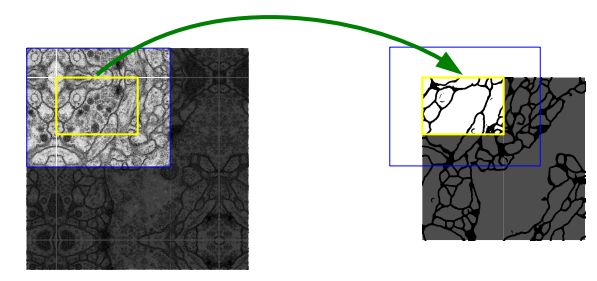
\includegraphics[width=.6\linewidth]{files/unet/tile.png}
	\caption{This is example of neuronal structures segmentation. It shows the overlap-tile strategy for seamless segmentation of large images. The yellow area is target for prediction and data inside the blue area is required as in input for prediction. Missing input data is exptrapolated by mirroring \cite{ronneberger2015u}.}
	\label{fig:tiling}
\end{figure} 

The right part of Figure: \ref{fig:U-net} illustrates the expansive path where every step consists of upsampling of feature map which is followed by a 2x2 convolutional operation (also referred to as up-convolution). This halves the number of feature channels. The gray arrow shows the concatenation of corresponding feature map from contracting path where it is cropped from the image. It is then subjected to two 3x3 convolutions and each followed up by a ReLU activation function. The cropping is required because of loss of boarder pixels during convolutions. At the final layer a 1x1 convolution maps each 64 component feature vector to the target number of classes i.e. background class and crater class. The final layer follows up by sigmoid activation function which determines the output of a class score between 0 to 1. Finally, binary cross entropy determines the loss while training of algorithm. In this model the total number of convolutional layers amounts to 23. It is important to select the input image size so that max pooling operations are applied to a layer with the same x and y size. This allows seamless tiling of segmentation map in output as shown in Figure: \ref{fig:tiling}

\begin{figure}[ht!]
	\centering
	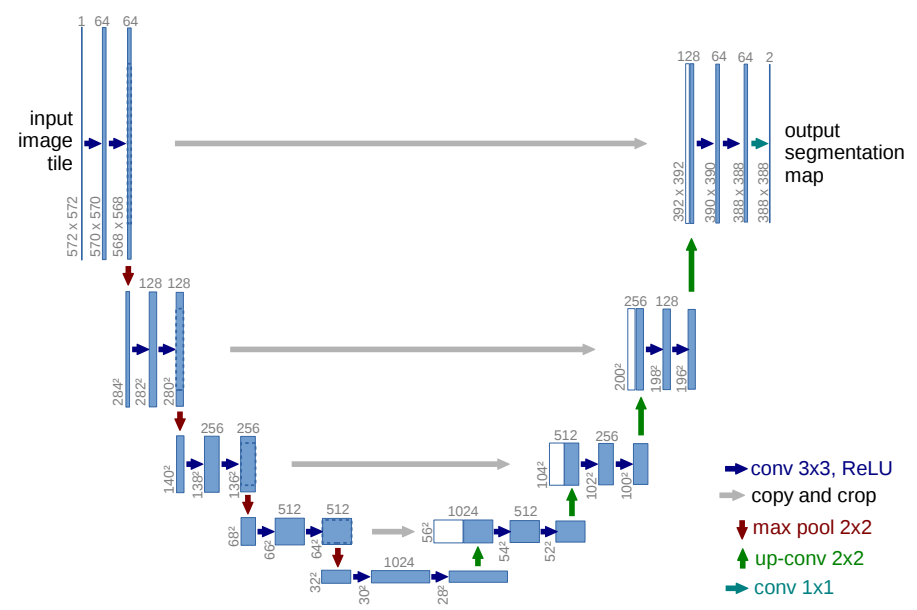
\includegraphics[width=.7\linewidth]{files/unet/arch.png}
	\caption{U-net Architecture \cite{ronneberger2015u}.}
	\label{fig:U-net}
\end{figure} 

\subsection{Convolutional Layer}
Convolutional layers essentially extracts a feature map from images. Images are mathematically represented by matrices with three color channels as red, green and blue (RGB). Gray scale images have only single channel. Therefore an image has a size $h \times w \times d$ where $d$ is depth represented by number of channels. Convolutional layers includes a filter (also referred to as kernel) which is also composed of $f_h \times f_w \times d$. Filter has a height and width smaller than the image size. It slides over (convolves with) the image producing a feature map. This convolution is the sum of element-wise multiplication of filter with the image. It is to be noted that depth of the filter is same as that of the input image therefore it varies with network.

Filter stride is a parameter that needs to be defined before training in convolutional layers. It determines the number of pixels by which a filter shifts at a time. Convolutional layers tend to reduce the output mapping size. A larger stride size will also result in a smaller sized output. Equation shows the relationship between output and input size of an image with a stride $s$ and filter $f$. The size of feature maps decreases by increase in convolutional layers. Row ($O_x$) and column ($O_y$) output size of convolutional layers are calculated as:

\begin{align}
O_{x}=\frac{i_{x}-f_{x} + 2p}{s}+1, \\
O_{y}=\frac{i_{y}-f_{y} + 2p}{s}+1
\end{align} 

Assuming example of an input image with size ($256 \times 256$) and a filter size of ($3 \times 3$) having a stride $s$ of 1 and zero padding $p$ will result into an output size of ($254 \times 254$). By using additional filters $n$, the feature map will be of size ($254 \times 254 \times n$). So, addition of filters will increase the output depth of a convolutional layer.

\begin{comment}
Lets suppose there is a 2D input image of size 6x6. A filter convolves through the image to extract an output image with desired features. The filter (which is also a matrix) could be of size lets say 3x3, extracts certain features of the image. This process is known as convolutional operation because filter convolve through the image.
\end{comment}

Example shown in fig: \ref{fig:Convolutional Operation} represents a typical convolutional operation without padding and stride of 1. The output 429 in 4x4 matrix is obtained by addition of element wise multiplication of the filter with top left 3x3 portion of the input image. Then filter jumps to next pixel and other values are obtained the same way.

\begin{figure}[H]
	\centering
	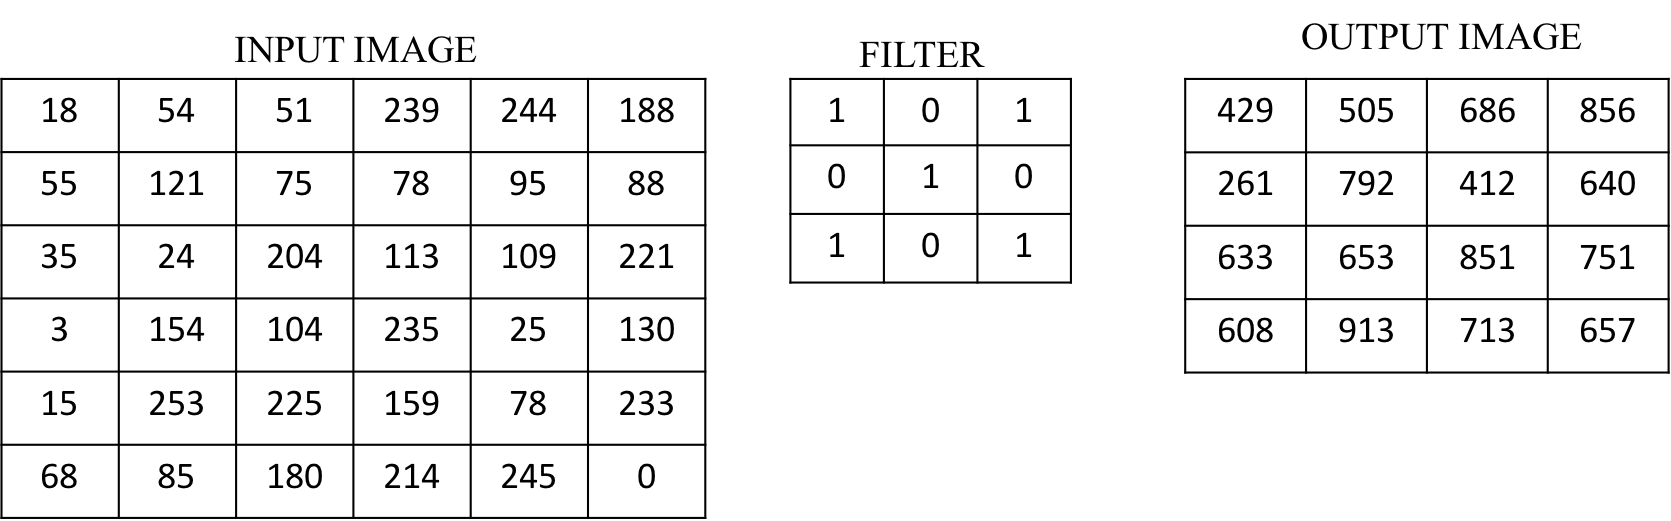
\includegraphics[width=.6\linewidth]{files/cnn_architecture/conv.png}
	\caption{Convolutional Operation}
	\label{fig:Convolutional Operation}
\end{figure}

\begin{comment}
\begin{equation}
\frac{n+2p-f}{s}+1 \times \frac{n+2p-f}{s}+1
\end{equation}

In the above example $n$ equals 6 as image is 6x6 and $f$ is 3 because of 3x3 filter size, $p$ is padding which equals 0 and $s$ stands for stride which is 1, inserting values in this equation would give us the size of output which is a 4x4 matrix.
\end{comment}

\subsection{Pooling Layer}
An input image could be large which increases the amount of parameters and introducing a pooling layer helps to reduce the number of parameters. Most commonly used type of pooling is max pooling. Fig \ref{fig:Pooling Operation} shows an example of max pooling with stride and filter size of 2. The idea is to keep the high values in each quadrant because the highest number represents a particular feature and in the example shown in Fig \ref{fig:Pooling Operation}, number 6 is the highest value in this quadrant. It means that the most activated pixel in this quadrant is 6 and same goes for other quadrants. The high values are preserved and lower ones are dropped out which are not as activated. Another pooling layer type is average pooling where averaged output of all the pixels is preserved. As it can be seen in the example below that pooling has reduced a 4x4 matrix to just 2x2 matrix, significant amount of parameters are reduced, in addition pooling may also help in reducing overfitting. The resultant matrix after a pooling operation can be obtained from the eq.(1) 

\begin{figure}[H]
	\centering
	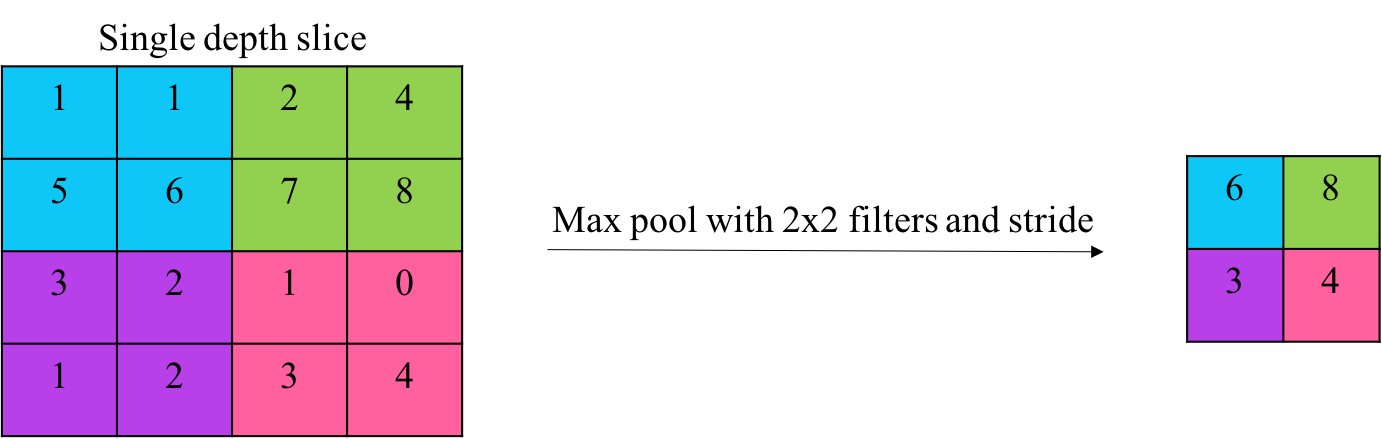
\includegraphics[width=.6\linewidth]{files/cnn_architecture/pooling.png}
	\caption{Pooling Operation}
	\label{fig:Pooling Operation}
\end{figure}

\subsection{Activation Functions}
These functions are an extremely important feature of a neural network. These functions decide which neuron (a neuron is noting but a mathematical function) would be activated. This means whether the information received by a neuron is relevant or should it be ignored. An activation function performs a non-linear transformation on the input signal and forward it as an input to the next layer of neurons.

Without activation functions weights and bias would be simply doing a linear transformation and a linear equation is easy to solve but very limited to the capacity of solving complex problems. Therefore, a neural network without having an activation function is nothing but a linear regression model which will not be capable of learning or performing complex tasks. Image classification or object detection is a complicated task and would require non-linear transformations. These functions make the process of back propagation possible because of the receiving gradients and error which are a measure to update weights and biases.

\subsubsection{Sigmoid Activation}
It is defines as:

\begin{equation}
a = \sigma(z) = \frac{1}{1+e^{-z}}=\frac{e^{z}}{e^{z}+1}
\end{equation}

where

\begin{equation}
z = Wx_i + b
\end{equation}

$W$ being weight vector and $x_i$ is image vector, $b$ stands for bias

The maximum output of this function is 1 and minimum is 0. Output always lies between values 0 and 1. Plotting a graph of sigmoid function represents it output more clearly:

\begin{figure}[ht!]
	\centering
	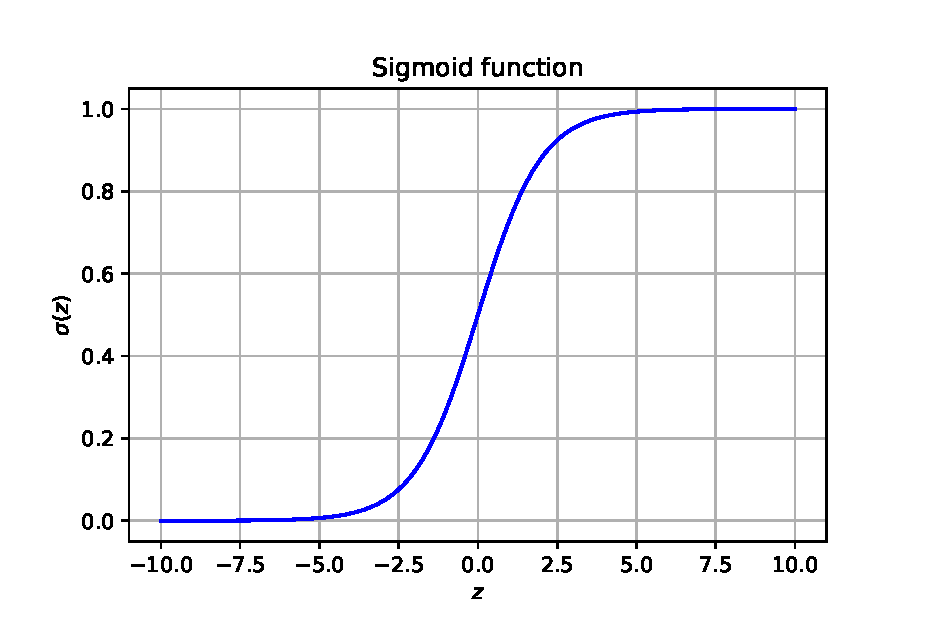
\includegraphics[width=.6\linewidth]{files/cnn_architecture/sigmoid.eps}
	\caption{Sigmoid Function}
	\label{fig: Sigmoid}
\end{figure}

From the graph it can be seen in the graph that $z$ is 0 when curve is passing though 0.5. In convention a rule can be set if i.e. $z$ is greater than 0.5 then output is always 1 and if less than 0.5 then it is 0. A notable behavior of this function is that if $z$ is larger than the dotted region in graph then the derivative of this function is close to zero and same way if it is negative slope is again equal to or close to zero. 

This means that it can slow down gradient descent. It also becomes a source of vanishing gradient problem. If the weights are initialized with either very large or very small values then these values saturate the input to sigmoid at very valued region (close to zero or close to one). Even if weights are initialized at a value i.e. ~0.2, in a deep network with many layers it will also lead to vanishing gradient problem. In case of only 4 layer network $0.2^{4}=0.0016$ which is small and will get even smaller in next layers. Also the mean of data is 0.5 which meas that data is not centered for the next layer. 

It is used for a problem where binary classification is required. In a neural network layer sigmoid must not be used in every layer because of the problems mentioned above. Anyhow, where binary classification is required, it can be useful in the last layer of the network to squash output such as $ 1 \geq \hat{y} \geq 0$.

\subsubsection{ReLU Activation}
It stands for rectified linear unit and defined as:

\begin{equation}
a = \max (0, z)
\end{equation}

The graphical form is given as:

\begin{figure}[ht!]
	\centering
	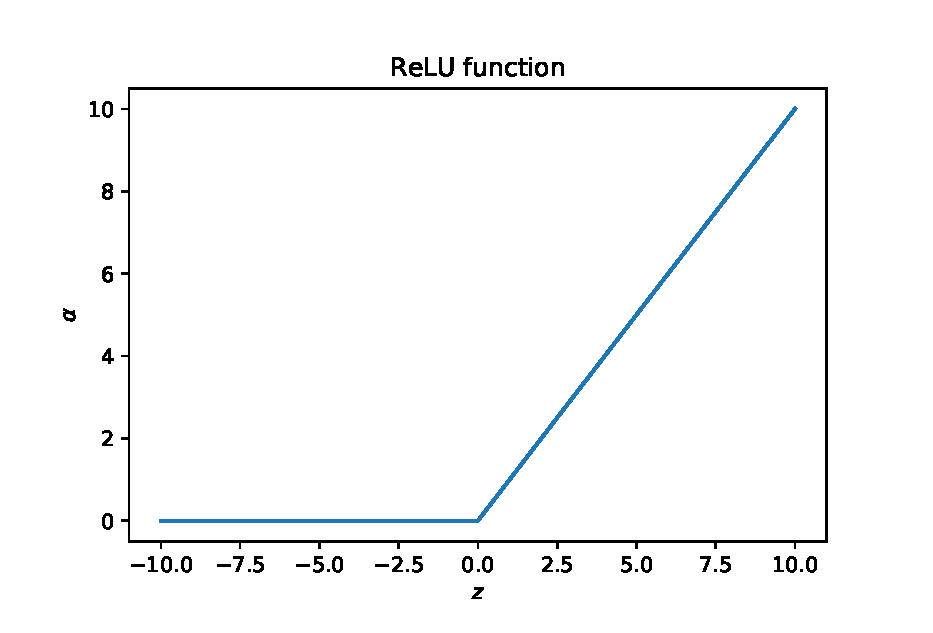
\includegraphics[width=.6\linewidth]{files/cnn_architecture/relu.eps}
	\caption{ReLU Function}
	\label{fig: relu}
\end{figure}

As seen in the graph ReLU gives an output for a positive value and otherwise the output is 0. It is to be noted that in graph the line looks linear but ReLU is non-linear in nature and it is one of most popular functions used in neural networks because of its simplicity and ability to not let all the neurons fire at once. ReLU is computationally much faster than sigmoid or tanh (written as $a=\tanh (z)$), it does not have exponent computation in such as sigmoid activation function therefore reduces training time significantly in very deep neural networks. \cite{krizhevsky2012imagenet} observed that training deep CNNs with ReLU is much faster as compared to sigmoid or tanh.

Unlike sigmoid when the receiving input is at the right or left plateau i.e. less than -5 or greater than 5 in Figure: \ref{fig: Sigmoid} which makes it meaningless to pass a backward pass because of derivative being closer to 0, ReLU only saturate when the input is a negative value. ReLU allows training of larger nets at much less computational costs which means more parameters can be trained at the same computational cost.

\subsection{Backpropagation}
A CNN requires to update its weight for a given training data in order to reduce loss. Backpropagation is an efficient method for computation of gradients which are required for gradient based optimization of weights or kernel parameters in neural networks \cite{rumelhart1988learning}. This optimization problem refers to minimize the loss function which is performed by the specific combination of weights. Backpropagation requires the computation of loss function at each iteration therefore loss function should be differentiable and continuous.

Initial weights of an untrained network are randomly taken. Without training a network is not able to make meaningful predictions for an input as there is no relation between an image and its groundtruth output yet. The weights in a network are adjusted by exposing a network to training samples which are labeled according the correct class. Before backpropagation there is a forward pass in which an image is taken into the network and first layer of network computes a feature map which is a very low level feature map. Then this activation map is fed to the next layer usually a hidden layer that computers another activation map with slightly high level features than the previous layer and this goes on till last layer yielding a network output. This results into a feature map which is determined by a loss function how much different it is from that of labeled feature. During backpropagation step of training the aim is to adapt weights in a way that difference between network output and desired output is minimized so that correct features can be extracted from an input image. There are usually multiple epochs till weights are adjusted so that loss is minimized. Backpropogation works on derivation chain rule to minimize loss function and all weights are updated in the negative direction of gradient function. A gradient is a vector containing derivatives. It is computed using partial derivatives and produces a vector field unlike a derivative which is dependent on a single variable. A Jacobian matrix represents gradient. Optimization algorithms such as Adam optimizer minimize or maximize loss function using its gradient values with respect to parameters.

Assuming a multiplication function of two numbers i.e. $f(x, y)=x y$, it is possible to derive the partial derivative for either of input:

\begin{equation}
f(x, y)=x y \quad \rightarrow \quad \frac{\partial f}{\partial x}=y \quad \frac{\partial f}{\partial y}=x
\end{equation}

The derivation function of a variable indicate the rate of change of a function with respect to that variable surrounding an infinitely small region near a specific point.

\begin{equation}
\frac{d f(x)}{d x}=\lim _{h \rightarrow 0} \frac{f(x+h)-f(x)}{h}
\end{equation}

In above equation the operator $ \frac{d}{d x} $ (a derivative operator) is applied to a function $f$. The resultant is a derivative. It can be interpreted as; if $h$ is very small then s straight line determines approximation of function and slope of the line is derivative. The sensitivity of an expression on a value is determined by the derivative. If $x=4, y=-3$ then $f(x, y)=-12$ and this would return a derivative on $x \frac{\partial f}{\partial x}=-3$. It is clear that if value of this variable is increased by a tiny amount, it would create an impact of three times decrement because of its negative sign. It can also be seen by rearranging the above equation such that; $f(x+h)=f(x)+h \frac{d f(x)}{d x}$. In other way as $\frac{\partial f}{\partial y}=4$, it is also expected that by increasing the value of $y$ by a tiny amount which is $h$ would also increase the function output by $4h$ because of positive sign.

\begin{comment}
The derivative of function $f(x,y)$ is a vector of partial derivatives which is $\nabla f=\left[\frac{\partial f}{\partial x}, \frac{\partial f}{\partial y}\right]=[y, x]$. Gradients can also be calculated for addition operation such as:

\begin{equation}
f(x, y)=x+y \quad \rightarrow \quad \frac{\partial f}{\partial x}=1 \quad \frac{\partial f}{\partial y}=1
\end{equation}

This indicates that derivative of both $x,y$ is one regardless of values of $x,y$. Increasing either $x$ or $y$ will increase the value of output to function $f$ independent of actual values of $x,y$ unlike the above case of multiplication. Another operation is a max operation:

\begin{equation}
f(x, y)=\max (x, y) \quad \rightarrow \quad \frac{\partial f}{\partial x}=1(x>=y) \quad \frac{\partial f}{\partial y}=1(y>=x)
\end{equation}

That is the gradient is 1 on the input which is larger and 0 on the other input. If $x = 4, y=2$, then max is $x$ and the function is not sensitive to value of $y$. If the value of $y$ is increased by a tiny amount $h$, the function will keep outputting value of $x$ which is 4, hence the gradient is 0. If the value of $y$ is changed by a large amount (in this case larger than 2) then output of $f$ will change. Derivatives shows nothing about the large changes on the function inputs. They only inform about the infinitely tiny amount of changes on the inputs as indicated in eq. 3.

Backpropagation relies on the above explained rule in a more complex neural network. It computes the gradient of loss function with respect to each weight via chain rule based on the above mentioned examples. The computation is performed one layer at a time starting from last layer till the second layer of network. First layer is not included as it is the input layer. Also redundant calculations are avoided by computing derivative of each layer at a time. In other words, the weights are adjusted every time in such a way that loss is minimized and the model reaches at a checkpoint where adjusted weights are very close to target features, hence to get most accurate predictions.

\begin{figure}[ht!]
\centering
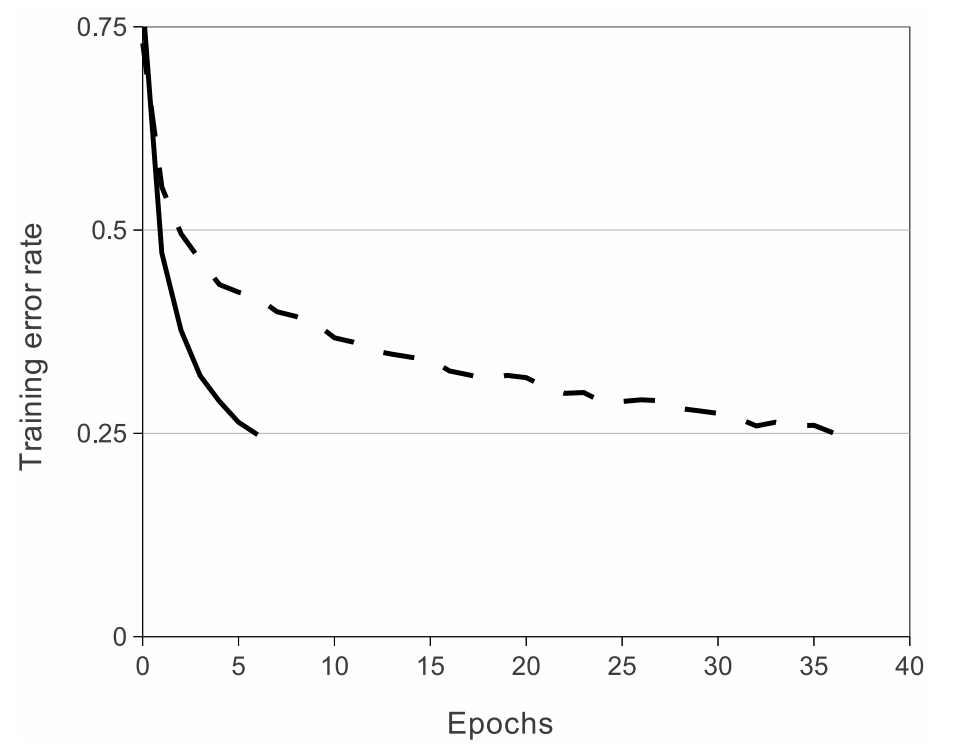
\includegraphics[width=.6\linewidth]{files/cnn_architecture/relu_fast.png}
\caption{A CNN of four layers trained with ReLU in solid line and tanh in dashed line. It shows that ReLU reaches a 25\% training rate on CIFAR-10 six times faster as compared to tanh \cite{krizhevsky2012imagenet}. }
\label{fig: relu_fast}
\end{figure}
\end{comment}

\subsection{Loss Function}
It determines the amount of deviation from the groundtruth or labeled data of the algorithm. Higher loss means the actual outcome is very different than expected result. A high loss function indicates poor performance of the model. If training is carried out in set of batches then a loss function is able to define the average of losses for individual training samples. 

There are different loss functions which are mainly chosen according to the type of problem. 

\subsection{Binary Cross-Entropy}
As the name suggests, it is a default loss function used for a binary classification problems. It is used where target values are 0 or 1. It calculates a score that summarizes the average difference between predicted and actual probability distributions for a predicting class 1. An ideal value for a cross entropy loss function is 0. Mathematically representation is given as:

\begin{equation}
H_{p}(q)=-\frac{1}{N} \sum_{i=1}^{N} y_{i} \cdot \log \left(p\left(y_{i}\right)\right)+\left(1-y_{i}\right) \cdot \log \left(1-p\left(y_{i}\right)\right)
\label{bce}
\end{equation}

Where $y$ is the label and $p(y)$ is predicted probability for $N$ points.

\begin{comment}

\subsubsection{Cross Entropy Loss}
It is also known as the log loss. It measures the performance of a classification model whose output is a probability value between zero and one. The cross entropy loss increases as the predicted probability diverges from the actual label so predicting a probability of i.e. 0.019 when the actual observation label is one would be bad and it would result in high loss value. Therefore, probability of observation as zero or one (positive or negative) is written as:

\begin{equation}
\label{crossent}
{\displaystyle H(p,q)=-\sum _{x}p(x)\,\log q(x)}
\end{equation}

In the above equation $p$ and $q$ are the cross entropy of true distribution and predicted distribution. The calculation of above equation depends on following factors:

\begin{enumerate}
\item Type of layers used in neural network.
\item Type of activation function used. Many activations might not be compatible with calculation because of output value which is either greater than one, negative value or do not sum to one. Therefore, softmax function is often used for multi class classification as it guarantees a well behaved probability distribution function.
\end{enumerate}

A machine learning, a common convention is to represent the ground truth (or labeled) data by vector $\mathbf{y}$ and $\mathbf{\hat{y}}$ is a vector containing the estimate. For a single example the equation is:

\begin{equation}
L = - \mathbf{y} \cdot \log(\mathbf{\hat{y}})
\end{equation}

If for example a true label is $\left[\begin{array}{llllll}{1} & {0} & {0} & {0} & {0}\end{array}\right]$ and predictions are $\left[\begin{array}{llllll}{0.1} & {0.5} & {0.1} & {0.1} & {0.2}\end{array}\right]$ then in this specific example all the probability is given to the first value and remaining are zero so they can be ignored. Mathematically it will be calculated as:

$$
\begin{array}{l}{L=-(1 \times \log (0.1)+0 \times \log (0.5)+\ldots)} \\\\ {L=-\log (0.1) \approx 2.303}\end{array}
$$

It is clear that loss would be same even if predictions are $\left[\begin{array}{llllll}{0.1} & {0.5} & {0.1} & {0.1} & {0.2}\end{array}\right]$ or $\left[\begin{array}{llllll}{0.1} & {0.6} & {0.1} & {0.1} & {0.1}\end{array}\right]$. This is a key feature of multi class cross entropy loss. The value does not depend on how probability is split between incorrect classes, it only penalizes the probability of correct class. 
\end{comment} 

\section{Experiments}
The experiments for crater detection are largely performed with U-Net based architecture however, a method of instance segmentation (Mask R-CNN) was also tested. As U-Net does not gives the intended output of crater counts and diameters, images are binarized according to various thresholding methods and for final outcome regional proposal algorithm was used on binary images. Hough circle transformation was also applied to find amount of craters directly from probability maps. Given below is the pipeline of crater detection process and details are discussed in sections given after.

\begin{table}[H]
	\centering
	\caption{Layers in U-Net}
	\begin{tabular}{|l|l|}
		\hline
		\multicolumn{1}{|c|}{Layer type} & \multicolumn{1}{c|}{Comments}                                                                                                                  \\ \hline
		\textit{\centering{Encoder}}                 & \multicolumn{1}{c|}{}                                                                                                                          \\[2ex] \hline
		Conv2D                           & Zero padding, ReLU activation                                                                                                                  \\ \hline
		Dropout                          & Value of 0.5                                                                                                                                   \\ \hline
		MaxPooling2D                     &                                                                                                                                                \\ \hline
		\textit{Decoder}                 &                                                                                                                                                \\[2ex] \hline
		UpSamplig2D                      & Size 2                                                                                                                                         \\ \hline
		Conv2D                           &                                                                                                                                                \\ \hline
		Dropout                          & Value of 0.5                                                                                                                                   \\ \hline
		Add                              & \begin{tabular}[c]{@{}l@{}}Adding the result of previous dropout with the \\ correspondingly sized Conv2D layer from encoder part\end{tabular} \\ \hline
		Final Layer                      &                                                                                                                                                \\ \hline
		Conv2D                           & Zero padding with sigmoid activation                                                                                                           \\ \hline
	\end{tabular}
\end{table} 

\subsection{Data Set}
There are two different datasets taken into account for model evaluation. First dataset which is in the form of gray scale lunar image is taken from lunar reconnaissance orbiter camera (LROC) archive \textit{http://wms.lroc.asu.edu/lroc/search}. Images from this data source are very large in size (5064$\times$52224) with resolution of 1.009. Which means processing these images would require a competitive hardware. Also each image in this data has several thousands of craters with sizes ranging from very few meters to several hundred meters. Keeping in view the size of an image and amount of craters present in an image, it was considered to take one of the image entitled as "M1111897809LE" (can be easily located in LRO database) and crop it into several small images of equal size and width (256$\times$256). This image has solar longitude angle of 52.81\textdegree. This cropping dimension was chosen based upon the ease for annotation process. Smaller image size would mean less craters to annotate in a single image and therefore more number of images in training set which would make data handling such as pre-processing and post-processing simpler. Initially the amount of cropped images were 300 out of which 240 are used for training and 60 are used for validation. For testing additional 20 images are annotated which makes the total annotation of 320 images with craters ranging from 1m to 200m diameters. 

Second dataset is taken from \cite{dino2020} who annotated an LRO gray scale optical lunar image with 21.36\textdegree{} solar longitude angle of the Apollo 17 landing site. The image is of the size 3130$\times$2427 pixels with resolution of 0.51 which is cropped into several images of the size 256$\times$256 for prediction. Tiles of this size are created to align this data with the testing data.

%hardware of 2 GPU NVIDIA GeForce MX150 and also the model is engineered to take input size of 256$\times$256 to limit hardware requirements.  

\begin{comment}
In machine learning normalization is a typical practice in preprocessing of data before its final preparation to run it through a neural network. Data can be standardized meaning subtracting a mean of dataset from each data point and dividing the dataset by standard deviation, mathematically standardization $z$ written as:
$$ z = \dfrac{x-m}{s}$$

Another way of normalization is to normalize a dataset by bringing it in a range of 0 to 1. This is typically true for image processing when pixels ranging from 0 to 255 which are normalized from 0 to 1. It is necessary to normalize data because without it some numerical data points can be very high and other might be very low. The larger data points in non-normalized datasets can cause instability in neural networks because the relatively large inputs can cascade down through the layers in the network which may cause imbalance gradients which may therefore cause the exploding gradient problem. This makes a network drastically harder to train and additionally significantly decrease training speed.

In neural network exploding gradient refers to a problem when weight is larger than identity and it is multiplied by pixels of image (ignoring bias in this case) then resultant is very high, this will further pass on to next neuron and it will be even higher, thus in a network specially in a deep network it will result into a very large value. The opposite problem is a vanishing gradient when a weight is less than identity then multiplication of weight results into even a smaller number therefore output is a very small value which means that network has barely learned in all of the layers.
\end{comment}

\subsection{Data Preparation}
For data preparation, annotation is one of the most important tasks in computer vision problem related to deep learning. This task is done manually, images are annotated and assigned a class. These are established by the annotator who can perform this task on the basis of simple instructions. No skilled labor is required to do this task. These annotations carry information to the neural network about the target features in an image. In this data. there is only one label which is "crater" and has shape of a circle, whereas rest is the background class.

Annotation or labeling could be laborious and time taking task. It is specially required when a network is not trained on the same type of class as required for predictions. In the case of lunar craters, there is not a great amount of work that has been done before in terms of deep learning therefore annotation was performed by me for training purpose. There are several annotation tools and after performing few experiments with various tools, VGG Image Annotator was found most simple and faster to annotate lunar crater data. This tool stores annotations in the form of a json format. Once the labeling is complete, a large json file represents the craters with a center point as $x$ and $y$ coordinates and radius respectively.

\begin{comment}
There are several tools to perform annotation, some are listed below.
\begin{itemize}
\item \underline{LabelMe}: One of the most commonly used tools. It has been observed that it is slow on UI mainly when zooming into images.
\item \underline{RectLabel}: At the time of annotation there was no support for Linux, it only worked for Mac.
\item \underline{LabelBox}: It provides options for different labeling tasks and works well for larger annotation projects.
\item \underline{VGG Image Annotator (VIA)}: Very simple design and easy to use for beginners as well as suitable for large projects as well.
\item \underline{COCO UI}: This tool for COCO dataset annotations.
\end{itemize}
\end{comment}

In Figure: \ref{an}, images in the first row are part of the training dataset and below them are the annotations. Images marked with circles on craters are not intended to be used for the training of algorithm, those are only visualizations to labeled data so that wrong annotations could be removed or missing ones could be added.

\begin{figure*}[ht!]
	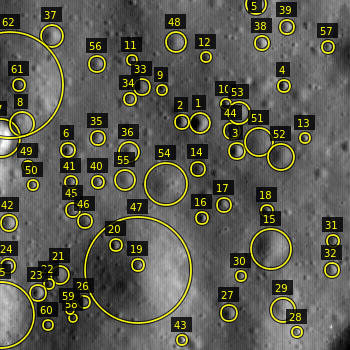
\includegraphics[width=.3\textwidth]{files/annotation/66n.png}\hfill
	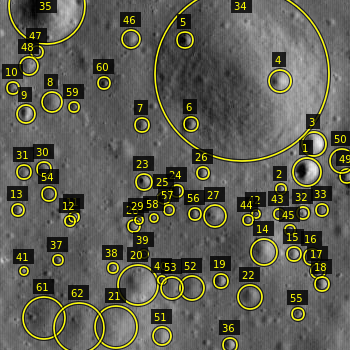
\includegraphics[width=.3\textwidth]{files/annotation/29n.png}\hfill
	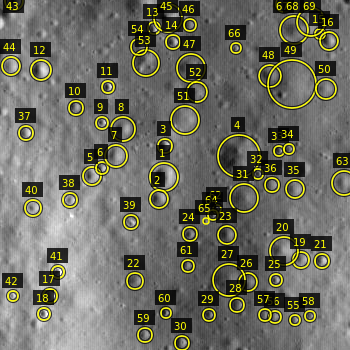
\includegraphics[width=.3\textwidth]{files/annotation/20n.png}
	\caption{Example of cropped images and corresponding labeled images. Annotation is performed using VIA tool}
	\label{an}
\end{figure*}

The result of these annotations is projected to get the masks of craters. These masks are binary images that represents the black and white pixel values of images. White pixels means craters and black means background class as shown in the Figure: \ref{mask}. White circles are craters belonging to Figure: \ref{an}. These provide learning objective to neural network that how the shape looks like and what features to learn. These binary masks have pixel values either 0 or 1 and are of the same shape along $x$ and $y$ as of the respective images.

\begin{figure*}[ht!]
	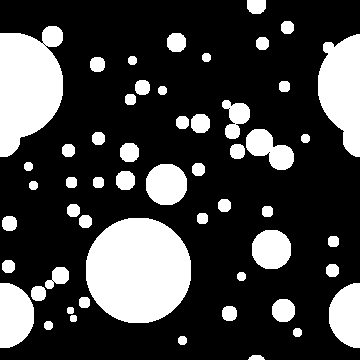
\includegraphics[width=.3\textwidth]{files/annotation/66m.png}\hfill
	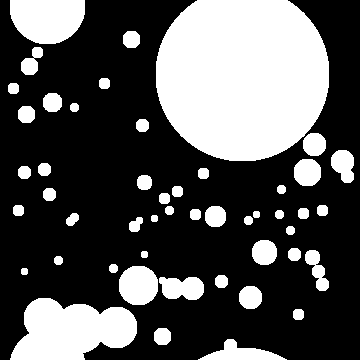
\includegraphics[width=.3\textwidth]{files/annotation/29m.png}\hfill
	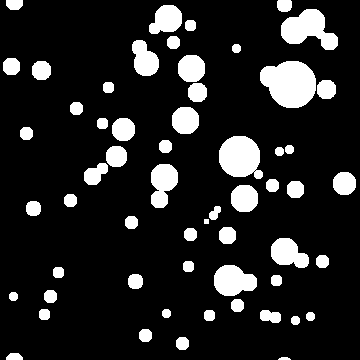
\includegraphics[width=.3\textwidth]{files/annotation/20m.png}
	\caption{Visualization of binary masks after projection from annotated (json format) images that belong to Figure: \ref{an}}
	\label{mask}
\end{figure*}

\subsubsection{Data Augmentation}
Reducing overfitting can be achieved through data augmentation. For many of the vision problems, generic input transformations like rescaling, cropping, adjusting colors or addition of noise are often helpful and may substantially improve generalization \cite{dvornik2019importance}. Development of more elaborate strategies requires prior knowledge of the task. For instance, all categories in ImageNet or Pascal VOC datasets are invariant to horizontal flips (e.g, flipping an airplane is still an airplane). But flipping will not be meaningful for the MNIST dataset, for example a flipped '5' is not a digit. Typically augmentation is achieved by creating new images with objects placed at various positions in existing scenes and this strategy of random placements has proven surprisingly effective for object instance segmentation \cite{dwibedi2017cut} which focuses on retrieving instances of a particular object. Where as in semantic segmentation the focus is on distinguishing categories rather than object themselves. For such tasks the random placement technique simply does not work and was proven through experimentation by \cite{dvornik2019importance}. 

Specifically for lunar optical image augmentation, training image is randomly augmented in following ways:

\begin{enumerate}
	\item \underline{Rotation}: Random rotation of images from $0^{\circ}$ to $360^{\circ}$ angle.
	%\item \underline{Translation}: Random change in shift in x and y direction of image between -4 to 4 pixels.
	\item \underline{Flipping}: Image is flipped with a factor of 0.5 as probability. 
\end{enumerate}

The images are randomly perturbed during training so that augmentation can have maximum effect. This way model have a low probability of seeing same type of training image more than once. In lunar crater dataset there are no RGB images hence color augmentation is opted out.

\subsection{Image Normalization}
Normalization is a key step in the preprocessing pipeline for any deep learning task. Normalization is also very important for lunar images and there are a variety of methods for doing this. The aim of normalization is to remove heavy variation in data that does not contribute to the prediction process and instead accentuate the features and differences that
are of most importance. Data normalization is an important step which ensures that each input parameter (pixel, in this case) has a similar data distribution. This makes convergence faster while training the network. As images are comprised of matrices with pixel values. Grayscale images are single matrix of pixels unlike colored images with three color channels. Normally pixel values range between 0 and 255. This raw format can also be used as an input to the neural network but this will increase amount of parameters that will result into slower training. Instead there is a great benefit in normalizing these pixel values to the range [0,1] to centering and even standardizing values. Lunar image data is normalized by subtracting the mean from each pixel and then dividing the result by standard deviation. The distribution of such data would resemble a Gaussian curve centered at zero. For image inputs, the pixel numbers should be positive, so the chosen scale to normalize each image pixel is in the range of [0,1]. 

\subsection{Training}
The data composed of images and their respective masks is divided into training (80\%) and validation (20\%) data set. This percentage practice is typical in machine learning, however it does not have to be always at this rate. In case of large data set i.e. several thousands of images, 60\% or even less can be set for training.

The input images along with their corresponding segmentation maps are utilized to train network with Adaptive Moment Estimation (Adam) implementation of Keras (originally written in Cafe \cite{ronneberger2015u}). Inside training pipeline, the convolutions are unpadded which leads to a smaller output size after every layer. This decrease in size is of the factor of constant border width. The batch size is reduced to a single image to minimize the overhead and utilize maximum GPU memory. In this configuration momentum is kept high (0.99) such that a larger number of already seen training samples determine the update in ongoing optimization step. Momentum helps to accelerate gradients vectors in the right direction. A softmax function over the final feature map combined with cross entropy loss function determines the energy function. In softmax which is defined as $p_{k}(\mathbf{x})=\exp \left(a_{k}(\mathbf{x})\right) /\left(\sum_{k^{\prime}=1}^{K} \exp \left(a_{k^{\prime}}(\mathbf{x})\right)\right)$, where $a_{k}(\mathbf{x})$ denotes the activation in feature channel $k$ at the pixel position $\mathbf{x} \in \Omega$ with $\Omega \subset \mathbb{Z}^{2}$. $K$ is the number of classes and $p_{k}(\mathbf{x})$ is the approximated maximum function. This means that $p_{k}(\mathbf{x})$ will be close to 1 for $k$ with maximum activation and vice versa for other values of $k$. The cross entropy function penalizes each deviation of $p(y)$ from 1 as defined in eq: \ref{bce}.

The weights are saved in a checkpoint when losses are less than previous saved checkpoint. Any of these saved weights could be utilized to apply on a test data set but definitely saved weights with best performance on validation data set is the best choice to be deployed on a test data set.

\subsection{Crater Detection Pipeline}
After training, to get detected craters from raw images, LRO large images are split into 256 $\times$ 256 sized tiles which goes through the following.

\begin{enumerate}
	\item Each 256 $\times$ 256 tile is fed to the segmentation network.
	\item Prediction results are stitched back together into the full sized original image. At this stage the resultant is a probability map which is also an image and can be compared to the target input image.
	\item To compute the radii and locations, binarization methods are applied to convert probability maps to binary images.
	\item The region proposal algorithm described by \cite{reiss1993recognizing} is used for computation of locations and radii from binary images.
	\item The model performance is evaluated by the F1 measure on test data from dataset split and data annotated from \cite{dino2020}.
	\item Neukum production function is used to plot CSFD against crater diameters and lunar age for the test data surface is estimated.
\end{enumerate}

\subsection{Prediction}
The best checkpoint of trained model is used for prediction on test data set. Prior to predictions the optical images are subjected to CLAHE for better results (more craters in a probability because of sharper contrast between craters and background). Predictions yield a probability map of each image in which light pixels depict maximum likelihood and darker ones represents low probability of crater existence. Such heat map of one of the test images is shown in binarization methods. Trained model is used for prediction on two test sets. First one is similar to training data set but test images are not seen by algorithm during training or evaluation. Second test data set (geographic location of Apollo 17) is annotated by \cite{dino2020} having a different sun illumination angle than first test data set.

Apart from region proposal algorithm, Hough circle transformation is also used for circle fitting but overall results are poor. It does a reasonable job of detecting some of large or medium-sized craters but overall performance is quite bad compared to SVM and CSTM \cite{wetzler2005learning}. Hough circle fitting on one of the test images can be visualized in Figure: \ref{hough}.

\subsection{Post-processing}
The resulting predictions from CNN model which are in the form of probability map are post processed, in this step images are first binarized (converted to white and black pixels) by applying various binarization methods which are discussed in binarzation section. This is needed in order to count number of craters and their diameters. Region proposal algorithm proposed by \cite{burger2009principles} is used for finding $x$, $y$ coordinates and diameter of craters along with the location in an image. The age of Apollo 17 region is already known. Therefore by identifying CSFD and crater diameters it is possible to estimate age which is plotted in a log-log plot and can be compared with dating performed by planetary scientists.

\subsection{Results and Discussion}
The intermediate results of final outcome are shown in figures below. The probability maps are the prediction of craters from optical input images. Several binarization methods are experimented on probability maps that have different threshold values. These differences can be easily visualized in binary images as varying quantities of white blob type objects.  

\begin{figure}[H]
	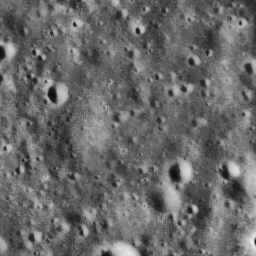
\includegraphics[width=.3\textwidth]{files/results/26.png}\hfill
	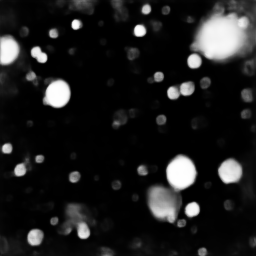
\includegraphics[width=.3\textwidth]{files/results/26_predict.png}\hfill
	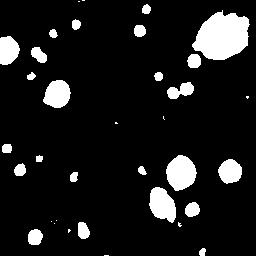
\includegraphics[width=.3\textwidth]{files/results/otsu.png}
	\caption{Otsu thresholding. Right most image is the thresholded image of the predicted probability mapped image of the middle. Most left is the actual image.}
	\label{otsu thresholding}
\end{figure}

\begin{figure*}[H]
	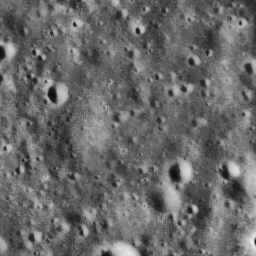
\includegraphics[width=.3\textwidth]{files/results/26.png}\hfill
	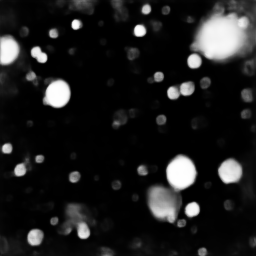
\includegraphics[width=.3\textwidth]{files/results/26_predict.png}\hfill
	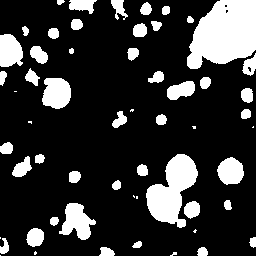
\includegraphics[width=.3\textwidth]{files/results/mean.png}
	\caption{Mean thresholding.}
	\label{mean_th}
\end{figure*}

\begin{figure}[H]
	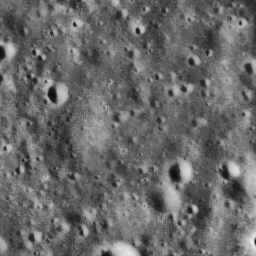
\includegraphics[width=.3\textwidth]{files/results/26.png}\hfill	
	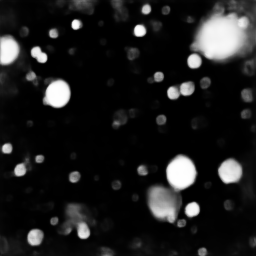
\includegraphics[width=.3\textwidth]{files/results/26_predict.png}\hfill
	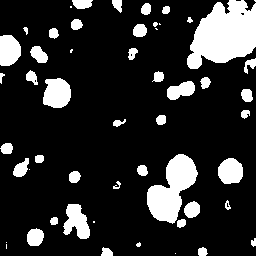
\includegraphics[width=.3\textwidth]{files/results/yen.png}\hfill
	\caption{Yen thresholding. Right most image is the thresholded image of the predicted probability mapped image in the middle. Most left is the actual image.}
	\label{Yen thresholding}
\end{figure}

\begin{figure}[H]
	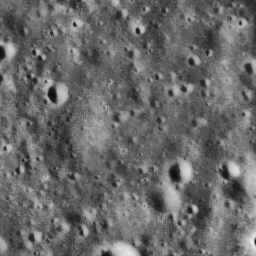
\includegraphics[width=.3\textwidth]{files/results/26.png}\hfill	
	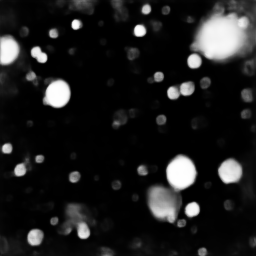
\includegraphics[width=.3\textwidth]{files/results/26_predict.png}\hfill
	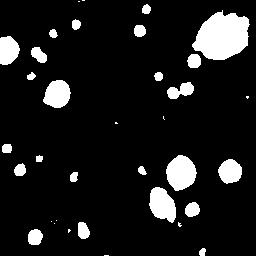
\includegraphics[width=.3\textwidth]{files/results/isodata.png}\hfill
	\caption{Isodata thresholding. Right most image is the thresholded image of the predicted probability mapped image in the middle. Most left is the actual image.}
	\label{isodata thresholding}
\end{figure}

\begin{figure}[H]
	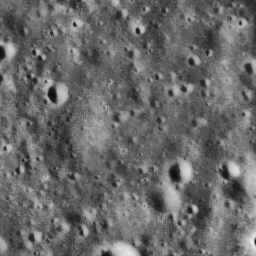
\includegraphics[width=.3\textwidth]{files/results/26.png}\hfill
	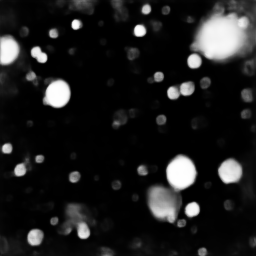
\includegraphics[width=.3\textwidth]{files/results/26_predict.png}\hfill
	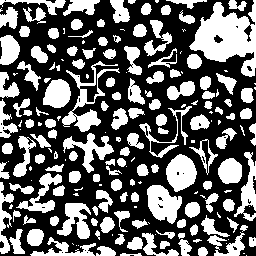
\includegraphics[width=.3\textwidth]{files/results/niblack.png}
	\caption{Niblack thresholding. Right most image is the thresholded image of the predicted probability mapped image in the middle. Most left is the actual image.}
	\label{Niblack_th}
\end{figure}

\begin{figure}[H]
	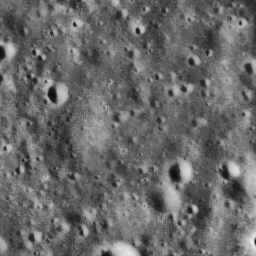
\includegraphics[width=.3\textwidth]{files/results/26.png}\hfill
	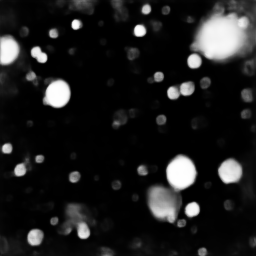
\includegraphics[width=.3\textwidth]{files/results/26_predict.png}\hfill
	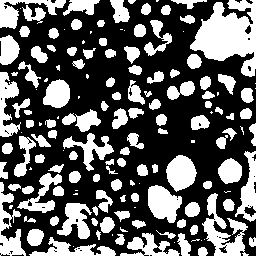
\includegraphics[width=.3\textwidth]{files/results/sauvola.png}
	\caption{Sauvola thresholding}
	\label{sauvola thresholding}
\end{figure}

\begin{figure}[H]
	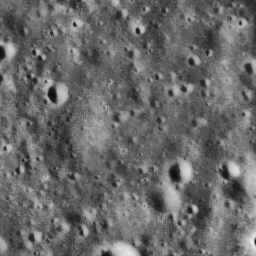
\includegraphics[width=.3\textwidth]{files/results/26.png}\hfill	
	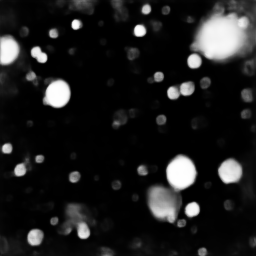
\includegraphics[width=.3\textwidth]{files/results/26_predict.png}\hfill
	\includegraphics[width=.3\textwidth]{files/results/adaptiveMean_mean.png}\hfill
	\caption{Adaptive mean thresholding. Right most image is the thresholded image of the predicted probability mapped image in the middle. Most left is the actual image.}
	\label{Adaptive mean thresholding}
\end{figure}

\begin{figure}[H]
	\includegraphics[width=.3\textwidth]{files/results/26.png}\hfill	
	\includegraphics[width=.3\textwidth]{files/results/26_predict.png}\hfill
	\includegraphics[width=.3\textwidth]{files/results/li.png}\hfill
	\caption{Li thresholding. Right most image is the thresholded image of the predicted probability mapped image in the middle. Most left is the actual image.}
	\label{Li thresholding}
\end{figure}

\begin{table}[H]
	\centering
	\caption{F1 scores on applied binarization methods on lunar crater probability map. First row shows the percent decrease (indicated with a negative sign) and percent increase of binarization method.}
	\begin{tabular}{l|l|l|l|l|l|l|l|l|l|l|l|}
		\cline{2-12}
		& -50 \% & -40 \% & -30 \% & -20 \% & -10 \% & 0\%   & 10\%  & 20\%  & 30\%  & 40\%  & 50\%  \\ \hline
		\multicolumn{1}{|l|}{Otsu}              & 51.9  & 53.3  & 53.0  & 51.7  & 52.8  & 51.9 & 50.7 & 50.1 & 47.9 & 46.7 & 45.9 \\ \hline
		\multicolumn{1}{|l|}{Isodata}           & 47.6  & 49.2  & 47.7  & 48.4  & 48.6  & 46.9 & 47.4 & 47.6 & 44.7 & 44.6 & 44.1 \\ \hline
		\multicolumn{1}{|l|}{Yen}               & 36.7  & 38.7  & 41.4  & 44.3  & 45.1  & 45.8 & 45.8 & 47.7 & 48.3 & 49.2 & 49.4 \\ \hline
		\multicolumn{1}{|l|}{Li}                & 36.7  & 38.7  & 44.2  & 44.4  & 45.2  & 45.8 & 45.8 & 48.2 & 48.4 & 49.5 & 49.3 \\ \hline
		\multicolumn{1}{|l|}{Mean}              & 32.5  & 35.1  & 36.0  & 36.7  & 38.8  & 40.1 & 42.6 & 44.4 & 44.6 & 46.0 & 45.8 \\ \hline
		\multicolumn{1}{|l|}{\begin{tabular}[c]{@{}c@{}}Adaptive\\ mean\end{tabular}}     & \multicolumn{11}{c|}{2.2}                                                                 \\ \hline
		\multicolumn{1}{|l|}{\begin{tabular}[c]{@{}c@{}}Adaptive\\ Gaussian\end{tabular}} & \multicolumn{11}{c|}{9.3}                                                                 \\ \hline
		\multicolumn{1}{|l|}{Sauvola}           & \multicolumn{11}{c|}{14.0}                                                                \\ \hline
		\multicolumn{1}{|l|}{Niblack}           & \multicolumn{11}{c|}{9.3}                                                                 \\ \hline
	\end{tabular}
\label{exp}
\end{table}

Experimental results given in Table: \ref{exp} are performed on \cite{dino2020} data. The data set consists of a single image of the size 3130x2427 pixels and it is cropped into several 256x256 images for predictions. Then prediction is performed on all the images and resulting predictions are concatenated together in an order similar to the original image. Then the experiment presented in Table: \ref{exp} shows computation of F1-score on several binarization techniques to find out which one yields highest F1-score.

It can be seen that the F1-score increases by increasing threshold for methods like Yen, Li and Mean but for Otsu and Isodata it decreases slowly by further increasing threshold. The thresholding methods result into slightly over or under segmentation in the case of crater detection. It can be seen that Otsu and Isodata results into a high threshold value thus by decreasing threshold it is likely that F1-score might increase. Rest of the methods results into over segmentation that specially penalizes recall thus resulting F1-score is lower in comparison. This makes sense and observed in experimentation.

Relationship between precision and recall of different filters is shown in Figure: \ref{thresh_methods}. Adaptive Mean, Adaptive Gausssian, Sauvola and Niblack are not shown in graphs because of their poor performance with respect to F1-scores as shown in Table: \ref{exp}. It is clear that by setting higher threshold reduces recall but increases precision. This can be observed from Otsu and Isodata methods as both results into higher threshold values. The difference between recall and  precision is obvious only if the segmenter is strongly over or under splitting \cite{badrinarayanan2017segnet}. In any of the case precision can be misleading as evaluation metric because it favors under segmentation. Contrary to precision, recall does not favor under or over segmentation, therefore F1-score is taken into account as the evaluation metric for segmentation accuracy. From graphs it can be noted that Otsu and Isodata provides a good trade off between precision and recall thus results into higher F1-score than other methods.
 
\begin{table}[H]
	\centering
	\caption{Patch wise mean F1 scores on test set distribution from dataset split}
	\begin{tabular}{c|c|c|c|}
		\cline{2-4}
		\multicolumn{1}{l|}{}         & Precision & Recall & F1 score \\ \hline
		\multicolumn{1}{|c|}{Otsu}    & 77.5      & 70.6   & 73.8     \\ \hline
		\multicolumn{1}{|c|}{Isodata} & 76.9      & 70.1   & 73.3     \\ \hline
		\multicolumn{1}{|c|}{Li}      & 56.9      & 80.5   & 66.7     \\ \hline
		\multicolumn{1}{|c|}{Yen}     & 51.8      & 72.9   & 60.5     \\ \hline
	\end{tabular}
\label{mine}
\end{table}

Table \ref{mine} shows the F1-score on 20 test images taken out from the same data set used for training. Computation is performed on each image separately then average of all the images is taken. Given filters are chosen on the basis of experimentation among different filters and their F1 comparison as given in Table \ref{exp}. It can be seen that Otsu has the best precision because of higher threshold value which yields less false positives. High threshold has a drawback of missing small craters which are usually less than 6 pixels and also those which are highly degraded and barely have a shadow. This can be seen by threshold of Li and Yen's method where recall is high but precision is punished. Overall, Otsu outperforms all the other binarization methods.

\begin{table}[H]
	\centering
	\caption{Patch wise mean F1 scores on a different test annotated from \cite{dino2020}}
	\begin{tabular}{c|c|c|c|}
		\cline{2-4}
		\multicolumn{1}{l|}{}         & Precision & Recall & F1 score \\ \hline
		\multicolumn{1}{|c|}{Otsu}    & 77.0      & 55.7   & 64.6     \\ \hline
		\multicolumn{1}{|c|}{Isodata} & 73.9      & 53.8   & 62.3     \\ \hline
		\multicolumn{1}{|c|}{Li}      & 60.7      & 59.2   & 59.9     \\ \hline
		\multicolumn{1}{|c|}{Yen}     & 51.9      & 53.1   & 52.5     \\ \hline
	\end{tabular}
\label{dino}
\end{table}

Table \ref{dino} shows F1 results on \cite{dino2020} data set. It is expected to see low F1-score compared to actual test set because of difference of shade length. Precision has not changed too much but there is notable decrement in recall score of methods and after analysing images visually, it is concluded that this happened mainly because of different sun illumination angle. Otsu once again outperforms other methods including Isodata by a slight margin.

It has been also observed that taking a large image, cropping it into 256$\times$256, performing predictions and stitching predicted images back together to form the actual image results into lower F1-score than computation on every image separately. This is due to the fact that many of the detected craters are split into half in two images and some are located in such a way that one image has crater shadow and other has illumination. This results into detection of crater on one image but not on the other, which means there is one true positive and one false negative so recall of the two images is 50\% instead of 100\%. That is why scores in Table \ref{exp} are much lower than Table \ref{mine} and \ref{dino}. It is also observed that cropping a large image and performing predictions on smaller cropped images will result into artifacts when segmented maps are stitched together. Binarization of stitched large image results into addition of false positives on reflection to artifacts which penalizes F1-score and has been observed in Table: \ref{exp}, therefore it makes more sense to perform image wise binarization and calculate F1-score on single image basis.

Mask R-CNN which is a deep neural network based architecture was also applied in experimentation. It is observed that performance of this architecture was poor despite of huge success on several types of object classification and instance segmentation problems. Analysis shows that this happened because of very little training data. Furthermore, Lunar craters does not resemble with classes the algorithm is trained on i.e. COCO or ImageNet data set. Moreover, the complexity of craters in optical images with shades on one side makes it difficult for such a deep architecture to learn from a data set composed of less than 300 training images. However, further research is needed to draw more explanation in this regard.
 
\begin{figure}[H]
	\begin{subfigure}{7cm}
		\centering\includegraphics[width=7.5cm]{files/results/otsu.eps}
		\caption{Otsu}
	\end{subfigure}
	\begin{subfigure}{7cm}
		\centering\includegraphics[width=7.5cm]{files/results/isodata.eps}
		\caption{Isodata}
	\end{subfigure}
	\begin{subfigure}{7cm}
		\centering\includegraphics[width=7.5cm]{files/results/mean.eps}
		\caption{Mean}
	\end{subfigure}
	\begin{subfigure}{7cm}
		\centering\includegraphics[width=7.5cm]{files/results/li.eps}
		\caption{Li}
	\end{subfigure}
	\begin{subfigure}[b]{1.0\textwidth}
		\centering
		\includegraphics[width=7.5cm]{files/results/yen.eps}
		\caption{Yen}
	\end{subfigure}

	\caption{Relationship between precision and recall on different binarization methods with upto 50\% increment and 50\% decrement from resultant threshold values at 10\% intervals.}
	\label{thresh_methods}
\end{figure}

\begin{figure}[H]
	\centering
	\includegraphics[width=.8\textwidth]{files/results/hcon_thesis-1.png}
	\caption{Five stitched prediction images of the size 256$\times$256 showing border artifacts.}
	\label{artifacts}
\end{figure}

Hough circle transformation was also applied for crater detection but the performance is very poor. One of the image is shown with several craters detected by the algorithm but Hough circle method extracted only 4 of them. This phenomena was also observed by \cite{wetzler2005learning} and his performance curves are given in Figure: \ref{roc,wetzler}.

\begin{figure}[H]
	\centering
	\includegraphics[width=.4\textwidth]{files/results/hough.png}
	\caption{Hough circle fitting on predicted image.}
	\label{hough}
\end{figure}

\subsection{Dating Lunar Surface}
Another evaluation is comparison of age with the determined age of crater counted surface by planetary scientists.

\section{Conclusion}
Crater automation can be challenging because of variability in appearance of craters and surrounding terrain. U-Net based architecture was applied to detect craters in optical images taken by Lunar Reconnaissance Orbiter. It is observed that by applying Contrast Limited Adaptive Histogram Equalization (CLAHE) the detection is increased up to 40\%. The resulting probability or heat maps were subjected to several binarization methods to create blobs for the lighter pixels in an image and Regional Proposal algorithm (implemented in scikit) was applied to detect blobs along with their respective diameters. Experiments show that Otsu's binarization method performs best even though Otsu's threshold creates an under-segmentation map. 

Several deep learning architectures have been applied to solve crater detection problem but largely are experimented with digital elevation models which eliminates small craters. In this thesis, U-Net was applied on optical images and it was tested on a proportion of dataset used for training and also on a different testset which is annotated by \cite{dino2020} with tighter solar longitude angle as compared to training dataset. An F1-score of 73\% was achieved on first testset whereas change in solar angle reduced F1-score to a value of 64\%.

%From the age estimation plot it can be seen that small craters with only 10 meters in diameter were also detected by U-Net. Introduction of larger dataset instead of data augmentation with different solar longitude angles might increase the performance of algorithm. 

\begin{comment}
\section{Cut}
These images could also be utilized for crater counting. Traditional methods of counting craters are manual by visual inspection of images. This approach is not practical when dealing large amount of images with craters of various sizes on either Moon or any other planet. This means that generated data is spatially comprehensive and restricted to largest craters or size comprehensive and limited to a specific geographic region \cite{stepinski2012detecting}. Manual crater counting by experts can result into disagreements as high as 40\% \cite{greeley1970precision}. Additionally, this requires skilled man power and time to find craters of various sizes across different geographical regions.
\end{comment}

\newpage
\clearpage

%%%%%%%%%%%%%%%%%%%%%%%%%%%%%%%%%

% Bibliography

%%%%%%%%%%%%%%%%%%%%%%%%%%%%%%%%%

	
\bibliographystyle{apalike}
\bibliography{mybib}

\end{document}
